\documentclass[10pt]{article}

\usepackage[a4paper,margin=2.6cm]{geometry}
\usepackage{amsmath,amssymb,amsthm}
\usepackage{array}
\usepackage{booktabs}
\usepackage{graphicx}
\usepackage{longtable}
\usepackage{microtype}
\usepackage[numbers,sort&compress]{natbib}
\usepackage[colorlinks=true,linkcolor=black,citecolor=black,urlcolor=black]{hyperref}

\newcommand{\NEO}{NEO}
\newcommand{\ORACLE}{ORACLE}
\newcommand{\GIC}{GIC}
\newcommand{\Bmat}{\mathbf{B}}
\newcommand{\bmat}{\mathbf{b}}
\newcommand{\Cmat}{\mathbf{C}}
\newcommand{\Fmat}{\mathbf{F}}
\newcommand{\Gmat}{\mathbf{G}}
\newcommand{\x}{\mathbf{x}}
\newcommand{\q}{\mathbf{q}}
\newcommand{\y}{\mathbf{y}}

\theoremstyle{definition}
\newtheorem{definition}{Definition}

\title{\NEO\ (Nonredundant Equivariant Orthogonalizer): Block-Local, Symmetry-Consistent Generalized Internal Coordinates for Molecular and Intermolecular Coordinate Spaces}
\author{Vincenzo Barone\\
INSTM, National Interuniversity Consortium for Materials Science and Technology\\
via G. Giusti 9, 50121 Firenze, Italy\\
\href{mailto:vincebarone52@gmail.com}{vincebarone52@gmail.com}}
\date{Working draft -- \today}

\begin{document}
\maketitle

\begin{abstract}
Internal coordinates are the natural language of molecular structure, yet their
automatic construction remains uneven across the use cases required by modern
spectroscopy and structure refinement.  Primitive redundant internals are robust
for geometry optimization but do not define a unique active space.  Global
non-redundant coordinates obtained from the singular-value or eigenvalue
decomposition of a full primitive Wilson matrix remove the redundancy, but the
resulting variables are often delocalized and sensitive to arbitrary weights
assigned to stretches, bends, torsions and non-covalent contacts.  Natural
internal coordinates provide the best chemical interpretation, especially for
force-field and vibrational work, but existing constructions are usually tied to
particular bonding patterns and do not provide a general, reproducible treatment
of fused rings, high coordination, point-group symmetry and weakly bound
fragments.

We present \NEO\ (Nonredundant Equivariant Orthogonalizer) as a general
construction of non-redundant, symmetry-adapted generalized internal
coordinates.  \NEO\ starts
from a frozen molecular state containing geometry, topology, atom equivalence,
point-group operations, fragments and optional interaction centers.  It then
builds chemically typed primitive families, protects special coordinates for
rings and fragments, reduces the coordinate space using analytic Wilson
\(\Bmat\)-row rank tests, and applies symmetry only inside homogeneous
coordinate blocks.  The result is a deterministic constructive protocol and a
frozen coordinate contract, rather than an arbitrary non-redundant basis.  The
contract can also incorporate optional user-defined protected semantic
coordinates and derived observables.  The same frozen definition is designed to
supply Gaussian-readable coordinates, analytic
\(\Bmat\) rows, symmetry labels and total-symmetric subsets for geometry
optimization, Wilson GF/potential-energy-distribution analysis, vibrational
scaling, force-field construction, discrete-variable-representation puckering
grids, potential-energy-surface fitting and semi-experimental
least-squares refinement.  A separate functional layer can then evaluate inverse or
exponential distance variables, trigonometric bend and torsional functions and
Cremer--Pople-like ring descriptors from the same base coordinates.  The method
therefore provides a constructive counterpart to natural internal coordinates:
it preserves their locality and interpretability while extending them to the
topological and symmetry cases that usually require manual intervention.
The numerical evidence reported here validates the construction invariants,
sparse derivative machinery and Gaussian export path.  We also discuss the
intended scope of the method and its current limitations.
\end{abstract}

\section{Introduction}

The Wilson internal-coordinate formalism gives a compact relation between
Cartesian displacements \(\Delta \x\) and internal-coordinate displacements
\(\Delta \q\),
\begin{equation}
  \Delta \q = \Bmat \Delta \x ,
\end{equation}
and remains the standard framework for vibrational analysis, potential-energy
distributions and internal-coordinate force constants.\cite{Wilson1955}  The
formalism itself does not solve the constructive problem: one must still choose
which coordinates define the molecular model.  That choice is benign in small
hand-built Z matrices, but it becomes a central scientific issue when the same
coordinate model is expected to support symmetry-constrained optimization,
semi-experimental structural refinement, ring puckering, weak complexes and
metal or high-coordination environments.

\NEO\ is designed to make this choice explicit and reproducible.  Table~\ref{tab:framework-roles}
defines the workflow names used below.  The essential separation is that
\NEO\ defines the non-redundant generalized internal-coordinate basis, analytic
Wilson matrix and symmetry labels; downstream modules choose how those
coordinates enter a fit, force field, scan or surface model.

\begin{table}[htbp]
\centering
\caption{Workflow components referred to in this manuscript.}
\label{tab:framework-roles}
\begin{tabular}{@{}p{0.18\linewidth}p{0.72\linewidth}@{}}
\toprule
Name & Role \\
\midrule
\ORACLE & Operator for Routing, Analysis, Control, Launch and Exploration; here,
the unpublished state layer used by \NEO.  It is a new implementation of the
continuous molecular perception ideas introduced in Proxima and of the synthon
descriptors used in previous templating-synthon work.\cite{Lazzari2020Proxima,Gambi2019Synthons,Lazzari2024SynthonPCS,Lazzari2025PCS141} \\
\NEO & Coordinate-generation engine: \GIC\ construction, symmetry-adapted
Cartesian reference spaces, analytic \(\Bmat\) rows, symmetry labels and
provenance. \\
GF/PED, DVR & Wilson GF/potential-energy-distribution analysis and discrete
variable representation. \\
MORPHEUS & Separate semi-experimental refinement workflow that motivates
coordinate persistence but is not validated in this paper. \\
\bottomrule
\end{tabular}
\end{table}

The novelty is not a new coordinate formula, but a deterministic constructive
protocol.  The central claim is not that a new Wilson matrix is needed.  It is
that a general coordinate generator must provide a deterministic
constructive protocol for choosing a non-redundant basis while satisfying four
requirements simultaneously.  First, the final variables must span the correct
vibrational rank, \(3N-6\) for nonlinear systems and \(3N-5\) for linear
systems.  Second, they must remain local enough to support chemical
interpretation, parameter constraints and force-constant analysis.  Third,
point-group symmetry must be applied without mixing unrelated coordinate types.
Fourth, non-standard but chemically important objects--ring puckering
components, ring-center distances, fragment translations and fragment
orientations--must be protected before ordinary valence coordinates fill the
remaining rank.  The result is not merely a coordinate list but a persistent
object that downstream modules can audit, reuse and compare against independent
active-space constructions.

Equally important, \NEO\ is not a new coordinate language.  Modern GIC
implementations already provide expressive syntax for nonlinear and mixed
coordinate expressions.  The novelty here is the preceding step: a
deterministic generator that converts a frozen molecular state into a
rank-complete, symmetry-consistent coordinate basis that can be serialized as
Gaussian-readable GICs or consumed directly by downstream modules.

The name \NEO\ uses ``equivariant'' in this classical molecular-symmetry sense:
coordinate rows are constructed so that point-group operations map them into the
same coordinate space with the corresponding atom permutation and vector or
pseudovector signs.  It does not denote a machine-learning equivariant model.
The acronym is also unrelated to nuclear-electronic orbital methods, which use
the same three letters for a different quantum-chemical context.
Likewise, ``orthogonalizer'' refers to normalized Wilson-row rank selection and
orthonormal SALC coefficient vectors within homogeneous source blocks.  It does
not claim global orthogonality in the kinetic \(\Gmat\) metric; that metric is a
downstream GF, DVR or refinement object.

\section{Relationship to Existing Coordinate Models}

Table~\ref{tab:context} summarizes the position of \NEO\ relative to the main
coordinate strategies used in quantum chemistry and molecular spectroscopy.
The comparison is deliberately constructive.  \NEO\ is not a replacement for
the Wilson formalism, natural internal coordinates or translation-rotation
coordinates; it is a general layer that decides how such ingredients are
assembled into one frozen, reusable coordinate object.

\begin{table}[htbp]
\centering
\caption{How \NEO\ is positioned relative to established coordinate strategies.}
\label{tab:context}
\begin{tabular}{p{0.20\linewidth}p{0.32\linewidth}p{0.37\linewidth}}
\toprule
Strategy & Strength & Limitation addressed by \NEO \\
\midrule
Z matrices & Compact, local and interpretable for small molecules. & Tree
dependence, singularities, and manual choices make them fragile for rings,
symmetry and automated workflows.\cite{BakerHehre1991ZMatrix} \\
Redundant internal coordinates & Robust for optimization and easy to generate
from a graph.\cite{PulayFogarasi1992,Peng1996Redundant,BakkenHelgaker2002} &
They do not define a unique active basis for vibrational analysis, symmetry
projection or least-squares refinement. \\
Delocalized internal coordinates & Automatic non-redundant bases can be
obtained from global rank decompositions.\cite{Baker1996Delocalized} & The
coordinates can mix stretches, bends, torsions and weak contacts; weights used
to control this mixing are method choices rather than chemical observables. \\
Natural internal coordinates & Highly interpretable symmetry and force-field
variables for well understood local motifs.\cite{Berces1997NaturalMetal,VonArnimAhlrichs1999GNIC,SwartBickelhaupt2006StrongWeak}
& General construction is difficult for fused or bridged rings, high
coordination, fragments, interaction centers and arbitrary point groups. \\
TRIC/geomeTRIC coordinates & Fragment translations and rotations give excellent
optimization variables for weakly connected systems.\cite{WangSong2016GeomeTRIC}
& Optimization coordinates are not by themselves a frozen, symmetry-labelled
internal-coordinate model for GF analysis or semi-experimental refinement. \\
Gaussian GIC syntax & Very general symbolic coordinate expressions, including
nontraditional geometric parameters, sparse derivative rows and automatic
symbolic differentiation, can be evaluated by an external optimizer; the recent
Gaussian implementation is the most direct general-purpose
comparison.\cite{Marenich2025GIC} & Standard internals can be generated from
connectivity and user-defined GIC expressions can be parsed and differentiated,
but the chemically specialized examples remain coordinates that are explicitly
specified in input or activated through dedicated options.  The syntax does not
define a complete natural-coordinate generator with protected rank reduction,
homogeneous point-group projectors and reusable symmetry-labelled blocks for
refinement or force-field analysis. \\
\NEO & Builds a rank-complete, type-labelled, symmetry-adapted coordinate basis
from a validated molecular state. & Weak complexes can be represented either
by protected fragment/center coordinates or by typed pseudo-bonds and
pseudo-cycles; the remaining development frontier is the breadth of the
pseudo-cycle validation corpus. \\
\bottomrule
\end{tabular}
\end{table}

This positioning is important for the narrative of the method.  Primitive
redundant internals and delocalized internals are excellent tools for geometry
optimization, where the main criterion is stable movement on a potential-energy
surface.  A semi-experimental fit or a Wilson GF analysis imposes stricter
requirements: the fitted or analyzed variables must be identifiable, symmetry
consistent and auditable as the same objects across independent modules.
Natural internal coordinates meet these requirements when the local chemistry is
known in advance.  B{\'e}rces extended their use to transition-metal skeletal
degrees of freedom,\cite{Berces1997NaturalMetal} von Arnim and Ahlrichs
generalized the automatic construction while still identifying multiply fused
ring systems as a hard case,\cite{VonArnimAhlrichs1999GNIC} and Swart and
Bickelhaupt emphasized the need to distinguish strong and weak coordinates in
optimization.\cite{SwartBickelhaupt2006StrongWeak}  \NEO\ turns this lineage
into a frozen construction for spectroscopy and refinement by combining
chemically typed primitive generation, block-local rank reduction,
special-coordinate protection and point-group projectors.

The recent Gaussian GIC paper is therefore the closest comparison and also
clarifies the remaining gap.  Its Supporting Information demonstrates the
power of the GIC language with nonlinear water coordinates, formamide
proton-transfer sum and difference variables, methane and ammonia
\(XY_3\)-type symmetrized combinations, polar and elliptic Li\(_2\)--Ar scan
variables, fragment rotor coordinates for benzene dimers and water clusters,
and quaternion fragment coordinates for ferrocene.\cite{Marenich2025GIC}
These examples clarify the distinction between an expressive coordinate
language and an automatic generator.  Gaussian can evaluate and differentiate
such expressions once they have been supplied or selected.  \NEO\ instead aims
to make the corresponding objects part of the frozen contract whenever they
follow from topology, local equivalence, point-group symmetry, fragments, ring
centers, bond centers or protected semantic coordinates.

This distinction is central to the positioning of the method.  Gaussian GIC is
an expressive coordinate-description language: a user can write arbitrary
primitive, nonlinear, redundant or mixed expressions and let Gaussian evaluate
them.  \NEO\ addresses a different problem.  It constructs the coordinate model
before any optimizer, force-field fit or refinement sees it, and records why
each protected or ordinary coordinate was accepted.  The Gaussian syntax is
therefore a serialization target for \NEO, not the theoretical object being
introduced.

In practical terms, the user should not have to write pages of molecule-specific
GIC definitions to obtain chemically natural variables such as local
\(XY_n\)-type combinations, proton-transfer sums and differences, fragment
translations or ring-puckering components.  When those variables are consequences
of the frozen molecular state, \NEO\ can generate and protect them
automatically; when they are requested explicitly, the request is recorded as a
semantic coordinate rather than as an opaque handwritten expression.

\section{Molecular State and Atom Equivalence}

\NEO\ does not rediscover the molecule at every downstream step.  Its input is a
validated \ORACLE\ molecular state containing Cartesian geometry,
covalent bonds, rings, point-group operations, optional fragments, optional
interaction centers and the continuous chemical perception produced upstream.
The output is a frozen \(\#\)GIC definition: primitive coordinate records,
final generalized coordinates, coefficients, family labels, irreducible
representations, total-symmetric subsets and the metadata required to
reconstruct analytic \(\Bmat\) rows.  Downstream modules consume this state;
they do not rebuild topology, ring sets or coordinate rows.

ORACLE is not yet a published program.  In the present manuscript it should be
read as the new molecular-state implementation used to provide \NEO\ with
published chemical descriptors: continuous molecular perception in the spirit
of Proxima,\cite{Lazzari2020Proxima} and molecular/spectral synthons developed
for accurate structural templating.\cite{Gambi2019Synthons,Lazzari2024SynthonPCS,Lazzari2025PCS141}
Initial local equivalence is therefore not based only on element symbols.  The
\ORACLE\ molecular-state layer supplies continuous atom perception and
synthon descriptors, and \NEO\ uses them to make deterministic local choices.
The present construction uses effective atomic numbers
that combine nuclear charge with local coordination, distance-derived
bond-order information, angular rigidity and delocalization-like terms.  These
continuous descriptors order atoms and ligands in cases where a pure graph
label would be ambiguous.  The broader \ORACLE\ topology layer also exposes
synthon descriptors--charge, covalency, delocalization, strain and effective
nuclear charge--which provide a natural route to more refined equivalence
classes.  In the present contract, this continuous perception enters ring
orientation, ligand grouping, local stretch equivalence, high-coordination
templates and the one-dihedral exocyclic torsion rule.
The determinism statements below are conditional on these descriptors being
part of the frozen input state.  In other words, \NEO\ does not assume an
unstated human perception step: the descriptor values, perception version,
topology and symmetry operations are stored as contract provenance, and a
change in any of them is a different molecular-state stratum.

\section{Coordinate Functions and Downstream Models}

The frozen \NEO\ basis is the first-order coordinate frame.  Many downstream
models, however, are better written in functions of those coordinates than in
the raw coordinates themselves.  This is especially true for force fields and
PES fitting, where the physically smooth variable may be an inverse distance,
an exponential contact coordinate, a trigonometric torsional term or a
ring-puckering descriptor.  We therefore distinguish base coordinates
\(\q\), which define rank and symmetry, from model coordinates
\(\y=f(\q)\), which are evaluated by downstream modules.

For any differentiable coordinate function \(y_a=f_a(\q)\), the Wilson row used
by a fit or force-field model follows from the chain rule,
\begin{equation}
  \label{eq:chain-rule}
  \frac{\partial y_a}{\partial \x}
  =
  \sum_i
  \frac{\partial f_a}{\partial q_i}
  \frac{\partial q_i}{\partial \x}.
\end{equation}
Thus the same frozen \(\Bmat\) service can support nonlinear coordinate
functions without changing topology, rank selection or symmetry labels.
Examples include \(r^{-1}\), \(\exp(-\alpha r)\) and damped contact functions
for distances; \(\sin\theta\), \(\cos\theta\), \(\sin n\phi\) and
\(\cos n\phi\) for bends and torsions; and Cremer--Pople-like \(q\) and
\(\phi\) descriptors derived from linear \(RPck\) components.  The same layer
also covers the practical variables used in the Gaussian GIC examples:
bond-sum and bond-difference coordinates for proton transfer, symmetrized
\(XY_n\) local combinations, polar or elliptic functions of intermolecular
Cartesian components, and quaternion or exponential-map functions of fragment
orientation.\cite{Marenich2025GIC}  In a GIC input language these are written
as explicit expressions or requested through a specific option; in \NEO\ they
are downstream functions of generated base coordinates or protected fragment
coordinates, with the chain rule preserving the connection to the frozen
Wilson rows.  Recent work by
Lema-Saavedra and Fern{\'a}ndez-Ramos shows why this separation is useful for
rings: Cremer--Pople amplitudes provide an efficient conformational search
space, while chemically viable 3D geometries require ring closure, angular
redistribution, treatment of rigid or multiple bonds and invariant local
references for substituents.\cite{LemaSaavedraFernandezRamos2026RingCP}  The
active Gaussian-readable coordinate basis should remain linear and rank
complete, while such nonlinear functions become named observables or model
variables in GF/PED, DVR, PES-fitting or refinement workflows.

Conformational reconstruction from puckering variables is therefore not external
to this workflow.  In the DVR layer, a one- or multidimensional grid in
\(RPck\)-, \(Q\)- or \(\phi\)-like variables must be associated with physically
closed ring geometries before electronic-structure points, metric terms or
wavefunctions can be interpreted.  The reconstruction layer of
Ref.~\citenum{LemaSaavedraFernandezRamos2026RingCP} provides precisely this
coordinate-to-geometry step: closure constraints, angular redistribution,
rigid-bond treatment and substituent reference frames belong above the frozen
\NEO\ basis, but they are natural consumers of it.  A DVR treatment can then
recompute the Wilson metric on the reconstructed structures, or use an explicitly
validated reduced metric, without introducing a second private ring-coordinate
definition.

This distinction also prevents a common ambiguity in the word ``GIC.''  A
general GIC expression can be an optimizer coordinate.  A \NEO\ coordinate
definition is a reusable coordinate contract: it specifies the base coordinate
space, the analytic derivatives and the symmetry transformation rules from
which later functional variables can be built.  Implementing these coordinate
functions systematically is part of the next development layer, but it does not
require a different coordinate-generation theory.

\NEO\ therefore exposes a small semantic coordinate layer rather than a second GIC
language.  \texttt{PROTECT} requests name base objects such as distances,
torsions, ring puckering, butterfly coordinates, fragment translations or
center distances.  Independent requests enter rank and symmetry selection with
the same priority as automatically generated protected coordinates.
\texttt{OBSERVABLE} requests define functions such as inverse distances,
trigonometric terms, linear combinations, Cremer--Pople variables or
proton-transfer coordinates; they are evaluated later as \(y=f(\q)\) by
Eq.~\eqref{eq:chain-rule}.  Duplicate protected rows are rejected,
row-equivalent user rows substitute the automatic primitive with provenance
recorded, and partial symmetry orbits are diagnosed before local SALC fallback.

\section{The Frozen Coordinate Contract}

The central output of \NEO\ is a frozen coordinate contract, not a transient
list of internal coordinates.  This distinction is important because the same
coordinate object must be used by independent modules, with no private
reconstruction of topology, symmetry or rank choices.

\begin{definition}
\label{def:frozen-contract}
A frozen coordinate contract is the tuple
\[
  \mathcal{C} = (\mathcal{P},\mathcal{G},\Bmat,\Sigma,\mathcal{M}).
\]
Here \(\mathcal{P}=(p_1,\ldots,p_m)\) is the ordered set of typed primitive
candidates; \(\mathcal{G}=(\mathbf{g},\Cmat_{\mathcal{G}})\) is the accepted
non-redundant generalized-coordinate basis together with its coefficient
matrix; \(\Bmat\) contains the analytic Wilson rows of the accepted basis;
\(\Sigma\) contains point-group transformation matrices,
irreducible-representation labels and SALC coefficients; and \(\mathcal{M}\)
contains the frozen molecular state, source-family labels, protection flags,
family priority order, numerical tolerances, semantic grammar and contract
schema versions, diagnostics and provenance.
Equivalently, with \(\mathbf{p}=(p_1,\ldots,p_m)^T\),
\[
  \mathbf{g}=\Cmat_{\mathcal{G}}\mathbf{p},
  \qquad
  g_a=\sum_{j=1}^{m} c_{aj}p_j,
  \qquad
  \Bmat=\frac{\partial\mathbf{g}}{\partial\x}
       =\Cmat_{\mathcal{G}}\Bmat(\mathcal{P}).
\]
\end{definition}

The tuple is the object consumed by GF/PED, DVR, PES-fitting and refinement
workflows.
It is also the object that makes the method auditable: a downstream result can
be traced to the primitive candidates that were generated, the rows that were
accepted or rejected, the rank tolerance that was used and the symmetry block in
which each final coordinate was projected.

Let \(X=\mathbb{R}^{3N}\) be the Cartesian displacement space and let \(T\)
denote the rigid-body tangent space generated by overall translations and
rotations.  For a nonlinear molecule, \(\dim T=6\); for a linear molecule,
\(\dim T=5\).  Scalar intramolecular coordinates have first-order rows in the
annihilator
\[
  X_{\mathrm{int}}^*
  =
  \{\ell\in X^*:\ell(t)=0\ \text{for all}\ t\in T\},
\]
whose target dimension is the vibrational rank \(r=3N-\dim T\).  Vector-like
fragment translations and orientations are stored as relative or body-fixed
generalized coordinates and are audited against the same external-mode-free
active space.  Each primitive candidate \(p_i\in\mathcal{P}\) contributes an
analytic row \(\bmat_i=\partial p_i/\partial\x\), and
\[
  \Bmat(\mathcal{P}) =
  \begin{bmatrix}
    \bmat_1 \\
    \vdots \\
    \bmat_m
  \end{bmatrix},
  \qquad
  \mathcal{R}(\mathcal{P}) =
  \operatorname{span}\{\bmat_1,\ldots,\bmat_m\}.
\]
The constructive goal is to choose an ordered subset
\(\mathcal{A}\subseteq\mathcal{P}\) such that
\[
  \operatorname{span}\Bmat(\mathcal{A})=\mathcal{R}(\mathcal{P}),
  \qquad
  |\mathcal{A}|=\operatorname{rank}\Bmat(\mathcal{P})=r ,
\]
when the primitive candidate set spans the full internal row space.  If this
condition fails, the build is not silently repaired; the contract records the
rank defect or excess and the molecular state must be reconsidered.

The novelty of \NEO\ lies in the constraints imposed on this basis selection.
The accepted set \(\mathcal{A}\) is not just any basis of
\(\mathcal{R}(\mathcal{P})\).  It is a chemically ordered basis selected under a
source-family preorder: protected fragment, center and ring coordinates are
tested before ordinary rank-completion candidates, and homogeneous chemical
families are reduced before unrelated families are allowed to compete.  This
replaces the search for an arbitrary non-redundant basis by the construction of
a basis with explicit semantic priorities.

\section{Construction Principles}

The construction is easiest to state as a sequence of constraints on the
candidate space.

\begin{enumerate}
\item All covalent bonds in the validated topology generate stretch candidates.
Stretches establish the bonded frame and are not allowed to be displaced by
later valence or torsional candidates.
\item Valence-angle candidates are generated locally around each bonded center.
When a center has equivalent ligands or high coordination, the candidate angles
are grouped by local equivalence or by recognized idealized coordination
templates before block-local reduction.
\item Exocyclic torsions are generated only for non-ring central bonds with
non-terminal substituents.  The default intramolecular path keeps one
representative torsional coordinate per exocyclic bond, selected by a CIP-like
priority based on the continuous effective atomic numbers and local
connectivity.  Symmetry-equivalent alternatives are averaged when they belong
to the same local orbit.
\item Endocyclic valence-angle and torsional source spaces are generated ring
by ring.  Their active combinations are not arbitrary lists of primitive
angles or dihedrals; they are block-local deformation and puckering components.
For an \(n\)-membered ring, the default active puckering source dimension is
\(n-3\), with Fourier-style component vectors and optional
bond-order-based flexibility factors.
\item Fused and condensed rings introduce additional torsional sources,
including butterfly coordinates around bonds shared by two rings.  These rows
remain in ring/torsional source blocks during reduction and symmetry
adaptation; they are not relabelled as generic torsions.
\item Special coordinates--fragment-center distances, center-atom distances,
fragment translations, fragment orientations and interaction-center distances--
are generated before ordinary candidates fill the remaining rank.  Their rows
are protected because they describe objects that ordinary valence coordinates
can span algebraically but not semantically.
\item The final non-redundant basis is selected by analytic \(\Bmat\)-row rank,
using a fixed family order and a protected-first policy.  Symmetry is applied
after a valid non-redundant basis exists, and only inside homogeneous source
blocks.
\end{enumerate}

This ordering differs from a global diagonalization of the full primitive
metric, whether expressed as \( \Bmat \Bmat^T \), as a row-space projector such
as \( \Bmat \Bmat^+ \), or as a single SVD of every redundant primitive at
once.  Such decompositions are mathematically useful, but their eigenvectors
depend on how the primitive rows have been scaled.  A stretch measured in
angstrom, a bend measured in radians, a torsion, a fragment translation and a
center distance have different natural units and different chemical roles.
Changing their weights can change which delocalized coordinates are retained.
\NEO\ instead uses rank-revealing linear algebra inside chemically homogeneous
blocks and reserves the final cross-block competition for a deterministic
analytic \(\Bmat\)-rank test.  This does not make the construction unique in an
abstract mathematical sense.  It replaces hidden numerical weighting choices by
an explicit chemical priority order whose provenance is stored in the frozen
definition.

\section{Primitive Families}

The primitive layer is intentionally redundant.  Redundancy is useful at this
stage because it allows chemical rules to create all plausible local
deformations before the rank selector removes dependent rows.  The important
restriction is that primitives are born with family labels that survive
reduction, symmetry adaptation and output.

\subsection{Bonded Coordinates}

Every covalent edge generates a stretch.  Equivalent stretches can be converted
to local sums and differences using a block-local SVD of their analytic
\(\Bmat\) rows, but the source block remains a stretch block.  Ordinary bends
are generated from pairs of neighbors around each center.  Nearly linear
centers produce two linear-bend components, because one ordinary angular
derivative becomes singular at linearity.

For three- and four-coordinate centers, \NEO\ uses local equivalence classes to
construct chemically recognizable bend combinations: symmetric deformations,
rocking coordinates and tetrahedral or \(WXY_3/W_2XY_2\)-like patterns.  For
coordination numbers between five and nine, the construction first attempts to match an
idealized local template; if no template closes reliably, ligand-equivalence
classes define the block that is reduced by SVD.  This is the practical
realization of the ``\(XY_n\) local symmetry'' idea: the algebra is local, the
grouping is chemically typed, and the result does not mix angle rows with
stretches or torsions.

\subsection{Exocyclic Torsions}

For an acyclic bond \(j-k\), all substituent pairs \(i-j-k-l\) are possible
primitive torsions.  Keeping every such torsion is usually unnecessary and can
create symmetry noise.  The default intramolecular path therefore uses the
one-dihedral rule: among non-linear substituent pairs, the selected pair is the
highest-priority pair under effective-atomic-number and local-connectivity
ordering.  If several pairs belong to the same local equivalence orbit, the
coordinate is the normalized average of the corresponding primitive dihedrals.
This gives one chemically stable torsional coordinate for each eligible
exocyclic bond while still respecting local degeneracy.
Here ``average'' means a stored linear combination of primitive torsional
Wilson rows, together with a scalar value on the branch fixed by the reference
geometry; it is not an arithmetic mean of periodic angles across a
\(360^\circ\) wrap.  When a finite torsional value is needed for reporting or
for a nonlinear model coordinate, \NEO\ uses the local reference branch, or an
explicit circular representation through \(\sin\phi\) and \(\cos\phi\).  Thus
symmetry averaging never identifies \(179^\circ\) and \(-179^\circ\) with an
unphysical zero-degree torsion.

\subsection{Rings, Puckering and Butterfly Coordinates}

Ring coordinates are the main place where primitive internal coordinates must
be replaced by natural combinations.  An \(n\)-membered ring has redundant
endocyclic angle and dihedral lists.  \NEO\ constructs ring deformation
coordinates and \(RPck\) puckering components as linear combinations of those
source rows, keeping \(n-3\) independent puckering components for rings larger
than three atoms.  The endocyclic valence-angle combinations are the CyGNA
source family and are stored as \(RDef\) rows; the corresponding endocyclic
torsional combinations are stored as \(RPck\) rows.  The polar
Cremer--Pople-like descriptors \(Q\) and \(\phi\) are useful for
interpretation, but the active coordinate basis stores linear \(RPck\) rows
because their \(\Bmat\) rows are analytic linear combinations of dihedral
derivatives.\cite{CremerPople1975}

For a six-membered ring segment \(1\cdots6\), a typical generated angle row has
the explicit form
\[
\begin{aligned}
RDef &=
 0.57735\,A(6,1,2)-0.28868\,A(1,2,3)-0.28868\,A(2,3,4) \\
&\quad +0.57735\,A(3,4,5)-0.28868\,A(4,5,6)-0.28868\,A(5,6,1),
\end{aligned}
\]
and the analogous puckering row is built from the corresponding cyclic
dihedrals with the same normalized coefficient pattern.  In the frozen
contract these rows carry family labels, source primitive identifiers and
symmetry labels; \(Q\) and \(\phi\) are then functions of the \(RPck\) rows, not
replacement active coordinates.

Unsaturated rings and locally rigid ring fragments require more than a generic
\(n-3\) puckering count.  The reconstruction method of Lema-Saavedra and
Fern{\'a}ndez-Ramos explicitly reduces the puckering dimensionality in the
presence of rigid or multiple bonds and then recovers the full ring geometry by
distributing the remaining distortions under constraints.\cite{LemaSaavedraFernandezRamos2026RingCP}
The present \NEO\ construction already introduces bond-order-dependent
flexibility factors in \(RPck\) source vectors, so dihedrals centered on more
rigid bonds contribute less to the puckering row.  The rigid-bond treatment of
Ref.~\citenum{LemaSaavedraFernandezRamos2026RingCP} is therefore most naturally
viewed in \NEO\ as a stronger, optional source-space contraction rather than as
a rewrite of the covalent graph.  A rigid bond \(i-j\) can be replaced, inside
that ring source polygon only, by the virtual source point
\(\mathbf{c}_{ij}=(\mathbf{r}_i+\mathbf{r}_j)/2\); the effective polygon then
has one fewer source point and one fewer puckering degree of freedom.  The
analytic \(\Bmat\) row is expanded back to the real atoms by the chain rule,
with the bond-center derivative distributed over \(i\) and \(j\).  This
contraction is attractive for genuine double bonds, conjugated fragments and
locally stiff fused-ring units, but it must be applied to complete symmetry
orbits and only when the \ORACLE\ continuous bond-order and synthon
descriptors mark a hard local constraint.  The present bond-order flexibility factors are
therefore the conservative default; rigid-source contraction is the planned
extension for cases where the chemically intended model removes, rather than
merely down-weights, a non-puckering motion from the active source space.  In
both cases, the active GIC basis remains linear while Cremer--Pople amplitudes
and phases are exposed as derived functions for sampling, PES fitting and
conformer classification.

Fused, spiro and bridged systems are handled as connected ring-source spaces
rather than as ordinary acyclic torsions.  When two rings share a bond, \NEO\
adds butterfly coordinates around that shared bond.  Condensed-ring torsions
and ring puckering components remain separate homogeneous blocks in the
symmetry projector.  This is essential for high-symmetry systems such as cubane
and for fused aromatic systems where a global torsion list would obscure the
local ring role.

\subsection{Out-of-Plane and Improper Coordinates}

Three-coordinate centers generate out-of-plane coordinates unless all four
atoms involved are cyclic.  Gaussian-compatible improper dihedrals can be
emitted in a compatibility mode, but the default analytic coordinate is the
out-of-plane \(U\) coordinate.  This distinction is an output convention, not a
change in the reduction policy: both forms occupy the same local
non-planarity role and are treated as their own coordinate family.

\section{Rank Reduction}

The rank-reduction step takes the ordered primitive set
\(\mathcal{P}=(p_1,\ldots,p_m)\), the analytic rows
\(\bmat(p_i)\) and a source-family map \(F:\mathcal{P}\to\mathfrak{F}\).
The family set \(\mathfrak{F}\) carries a priority preorder
\(\preceq_{\mathfrak{F}}\).  Protected families--fragment coordinates,
interaction-center distances, ring-puckering sources and related special
objects--are minimal elements in this preorder; ordinary stretches, bends and
torsions fill the rank only after protected rows have been tested.  Ties inside
a family are resolved by deterministic topology, \ORACLE\ equivalence and
CIP-like priority keys stored in \(\mathcal{M}\).  Thus the construction works on a
fixed total order that extends a chemically motivated partial order.

\paragraph{Relabelling covariance.}
\label{thm:relabel}
Let two frozen molecular states be related by an atom relabelling \(\pi\) that
preserves element identities, geometry, topology, \ORACLE\ descriptors, fragments,
interaction centers, point-group operations, priority keys and tolerances.  Let
\(Q_\pi\) be the induced orthogonal permutation of Cartesian displacement
coordinates and \(U_\pi\) the induced permutation/sign map on primitive
coordinate rows.  If \NEO\ returns a contract \(\mathcal{C}\) for the first
state, then it returns an isomorphic contract \(\pi_*\mathcal{C}\) for the
second state.  In particular,
\[
  \Bmat(\pi_*\mathcal{P})
  =
  U_\pi \Bmat(\mathcal{P}) Q_\pi^T,
\]
and the accepted coordinate spaces, family labels and symmetry-adapted blocks
are carried into each other by the induced row and coefficient-space
isomorphisms.
This follows because every primitive generator, row norm, rank residual and
homogeneous-block projector is evaluated from data preserved by \(\pi\);
orthogonal permutation/sign transformations do not change the Boolean
acceptance tests.

Equivalently, \NEO\ is natural with respect to symmetry-preserving atom
relabellings: relabelling the molecular state and then constructing the
contract gives the same object, up to the canonical contract isomorphism, as
constructing the contract first and then transporting it by the relabelling.

\paragraph{Deterministic coordinate contract.}
\label{prop:determinism}
For a fixed molecular state--geometry, topology, \ORACLE\ descriptors, point-group
operations and fragment data--and for fixed primitive generators, family
priority order, tie-breaking keys, row-normalization rule and numerical
tolerances, \NEO\ returns a unique frozen coordinate contract, or a unique
incompatibility certificate.  In particular, no stochastic search, optimizer
history or manual choice is part of the contract definition.
The verification is direct: each stage is a deterministic map of the frozen
input data, and the fixed order of candidate rows converts every rank and
symmetry decision into a stored threshold test.

\paragraph{Semantic preservation of protected coordinates.}
\label{prop:protected}
Let \(\mathcal{P}_{\mathrm{prot}}\) be the protected prefix of the ordered
candidate set.  Every protected candidate whose Wilson row is nonsingular and
independent, within the stored tolerance, of the previously accepted protected
rows is retained in any returned final contract.  No ordinary stretch, bend or
torsion can displace an accepted protected coordinate.  If the independent
protected prefix already exceeds the target vibrational rank, \NEO\ reports an
invalid contract rather than removing protected coordinates by exchange.
This is a consequence of the ordered-prefix construction: protected rows are
tested before ordinary rows and, once accepted, are never replaced by a later
exchange step.

\paragraph{Rank-preserving selection.}
\label{prop:rank-selection}
Assume exact arithmetic and define
\[
  \mathcal{R}_k=\operatorname{span}\{\bmat(p_1),\ldots,\bmat(p_k)\}.
\]
Incremental Gram--Schmidt selection accepts \(p_k\) exactly when
\(\bmat(p_k)\notin\mathcal{R}_{k-1}\).  After all candidates have been tested,
the accepted subset \(\mathcal{A}\) is an ordered basis of
\(\mathcal{R}(\mathcal{P})\).  If
\(\operatorname{rank}\Bmat(\mathcal{P})=r\), then
\(|\mathcal{A}|=r\) and
\(\operatorname{span}\Bmat(\mathcal{A})=\operatorname{span}\Bmat(\mathcal{P})\).
Indeed, at step \(k\) Gram--Schmidt decomposes \(\bmat(p_k)\) into its
projection on the current accepted span plus an orthogonal residual; a zero
residual leaves the span unchanged, and a nonzero residual adds exactly one
new independent direction.

The numerical construction is the finite-precision version of this statement.  \NEO\
selects rows by incremental modified Gram--Schmidt rank testing with a fixed
numerical tolerance, but the comparison is performed on normalized Wilson rows,
\begin{equation}
  \hat{\bmat}(p) = \frac{\bmat(p)}{\|\bmat(p)\|_2}.
\end{equation}
The residual tested for candidate \(p\) is
\begin{equation}
  \rho(p) =
  \left\|
    \hat{\bmat}(p) -
    \sum_{i \in \mathcal{A}}
    \left[\hat{\bmat}(p)\cdot \hat{\bmat}_i\right]\hat{\bmat}_i
  \right\|_2 ,
\end{equation}
where \(\mathcal{A}\) is the current accepted orthonormal row basis.  The
absolute row norm is used only to reject singular coordinates; independence is
decided by the direction of the analytic Wilson row.  This normalization avoids
a direct comparison of raw angstrom and radian scales in the final rank test.
It does not remove all modelling choices: the ordered candidate list remains a
chemical convention, not a theorem of uniqueness.  Singular rows and rows
dependent on previously accepted rows are recorded in the frozen diagnostics.

The decisive policy is therefore not only the linear algebra routine; it is the
priority constraint under which the basis is built.  Special protected
coordinates are tested before ordinary primitives.  Ordinary stretches, bends
and torsions then complete the rank.  A protected coordinate can be skipped only
if it is singular or dependent on previously accepted protected rows.  It cannot
be displaced merely because an ordinary valence coordinate spans a similar
first-order motion.  If independent protected coordinates alone exceed the
vibrational rank, the construction is rejected rather than silently discarding a
special coordinate.

\paragraph{Block-local scaling invariance.}
\label{thm:block-scaling}
Let \(H\subset\mathcal{P}\) be a homogeneous coordinate block.  Uniformly
rescaling all Wilson rows in that block by a nonzero scalar does not change the
normalized-row rank decisions inside \(H\), nor the singular-vector or projector
subspaces obtained from \(\Bmat_H\Bmat_H^T\).  By contrast, a global
decomposition of several heterogeneous blocks is generally not invariant to
independent rescalings of those blocks.
The reason is that row normalization removes a uniform factor inside \(H\), and
\((\lambda\Bmat_H)(\lambda\Bmat_H)^T=\lambda^2\Bmat_H\Bmat_H^T\) rescales
eigenvalues but not eigenspaces; concatenating heterogeneous blocks before
diagonalization changes their relative weights.

\paragraph{Local stability.}
\label{thm:local-stability}
Let \(S_0\) be a nonsingular frozen molecular state.  Assume that, in a
neighbourhood of \(S_0\), topology, fragment decomposition, \ORACLE\ equivalence
classes, point-group representation, protected prefix, homogeneous block
membership and priority order remain fixed in a ball of radius
\(\delta_{\mathrm{str}}\) around \(S_0\).  Let
\(\{f_a(\x)\}_{a=1}^{n_t}\) be the finite set of scalar decision functions used
by the construction in this stratum: row norms, rank residuals, block singular
or projected-vector norms and any sign-gauge pivot quantities used to store
SALC coefficients.  Let \(\tau_a\) be the corresponding acceptance threshold and
define the margin at \(S_0\)
\[
  \mu_a = |f_a(\x_0)-\tau_a| > 0 .
\]
Assume that each \(f_a\) is Lipschitz on the whole stratum ball with a uniform
constant \(L_a\), i.e.,
\[
  |f_a(\x)-f_a(\y)| \le L_a\|\x-\y\|
\]
for all \(\x,\y\) in that ball.  Then every
\[
  0 < \delta <
  \min\left[
    \delta_{\mathrm{str}},
    \min_{a:L_a>0}\frac{\mu_a}{2L_a}
  \right]
\]
preserves the discrete coordinate contract, with the usual convention that the
inner minimum is \(+\infty\) if all \(L_a=0\).  Thus every state \(S\) in the
same discrete stratum with \(\|\x(S)-\x(S_0)\|<\delta\) generates an isomorphic
coordinate contract: the primitive identities, accepted/rejected rank decisions,
protected coordinates, family labels and symmetry labels are unchanged, while
\(\Bmat\) rows and coefficient matrices vary continuously with the geometry
under the same normalization convention.
This is the usual finite-decision margin argument: each decision function stays
on the same side of its threshold for perturbations smaller than
\(\mu_a/(2L_a)\), and the minimum over the finite decision set preserves the
entire ordered construction.

This is the technical reason for block-local reduction.  \NEO\ does not claim
that weights disappear from all possible coordinate constructions.  It avoids
using arbitrary cross-family weights to define chemically labelled variables.
Only after homogeneous blocks have been reduced and protected coordinates have
been accepted does the final normalized rank audit compare directions across
families.

The local-stability result is deliberately stratum-local rather than global.  A
change in topology, symmetry, local equivalence or a near-threshold residual is
a genuine model change; it is therefore reported as contract provenance rather
than hidden behind a re-diagonalized global basis.

This policy is what makes the coordinate set suitable for refinement.  A
fragment-center distance or ring-center to atom distance might be expressible as
a linear combination of many ordinary internal derivatives near a reference
geometry.  That algebraic fact does not make the ordinary combination a useful
fit variable.  The protected-first rule preserves the variables that define the
model, then uses ordinary coordinates for completeness.

\section{Symmetry Adaptation}

Symmetry is applied only after a non-redundant coordinate basis has been
selected.  Let \(G_{\mathrm{pt}}\) be the molecular point group stored in the
source state.  The point group is not guessed from idealized element labels
alone: \ORACLE\ first clusters atoms by continuous element, coordination,
bond-order and synthon descriptors, then tests candidate rotations, reflections
and inversion operations against the Cartesian geometry within the stored
tolerances.  An operation is accepted only when it maps each atom onto an atom
of the same continuous equivalence class and preserves the stored topology and
local descriptor signatures.  The accepted operations, atom permutation table,
tolerances and perception version are frozen before \NEO\ constructs
coordinates.  Each operation \(h\in G_{\mathrm{pt}}\) is represented by a
Cartesian rotation matrix, an atom permutation and the signs required for
oriented coordinates such as torsions, out-of-plane bends and axial fragment
rotations.  For a homogeneous accepted coordinate block \(H\), with coefficient
space \(V_H\), the stored operations map the block into itself.  Since each
homogeneous block admitted to the projector is invariant under this permutation
and sign representation, its coefficient space carries a finite-dimensional
representation of the point group,
\[
  \Gamma_H:G_{\mathrm{pt}}\rightarrow GL(V_H).
\]
In the simplest case \(\Gamma_H(h)\) permutes equivalent coordinate basis
vectors and multiplies them by the appropriate parity sign.

If \(H\) is closed under the stored operations, the symmetry-adapted subspace of
irreducible representation \(\alpha\) is obtained by the standard character
projector
\begin{equation}
  \Pi_{\alpha}^{(H)}
  =
  \frac{\ell_\alpha}{|G_{\mathrm{pt}}|}
  \sum_{h\in G_{\mathrm{pt}}}
  \chi_\alpha(h)^*\,\Gamma_H(h),
\end{equation}
where \(\ell_\alpha\) is the dimension of \(\alpha\) and
\(\chi_\alpha\) its character.  \NEO\ applies these projectors to the coefficient
space of the block, orthonormalizes the nonzero projected vectors and stores the
resulting SALC matrix \(C_{\alpha H}\).  The symmetry-adapted Wilson rows are
then
\[
  \Bmat_{\alpha H}=C_{\alpha H}\Bmat_H .
\]
If an irreducible representation occurs with multiplicity greater than one in
the same homogeneous block, the projector defines a subspace, not a unique
printed basis.  \NEO\ fixes the stored basis by applying modified
Gram--Schmidt to projected source vectors in the canonical block order, by
discarding vectors below the saved norm tolerance, and by choosing the sign from
the largest-magnitude coefficient pivot.  The subspace is the representation
theoretic object; the ordered, sign-gauged coefficient matrix is the
deterministic serialization stored in the contract.
Along scans or optimizations, a change in the identity of the largest pivot can
flip the printed gauge even when the invariant subspace, rank and symmetry
labels are unchanged.  \NEO\ therefore treats pivot changes as executable path
diagnostics: consecutive SALC coefficient matrices are compared by subspace
overlap, pivot changes are flagged as gauge events, and the same diagnostic
module provides a Procrustes alignment for downstream GF/PED or DVR layers
when a path-continuous row basis is required.  None of the reported
chair-to-boat, ferrocene or GF/PED probes showed a pivot switch in the active
blocks used for the tabulated quantities.

The homogeneous-block rule is the key safeguard.  A stretch and a torsion may
belong to the same irreducible representation, but they are not the same kind
of coordinate.  Mixing them during symmetry adaptation would produce a valid
vector in an abstract representation and an opaque variable in a chemical
model.  \NEO\ therefore projects only within coordinate families and source
blocks.  If a block is not closed under the stored operations, the construction uses
an explicit local SALC fallback only where the contract allows it, and records
that fallback in the symmetry diagnostics.

Fragment translations transform as polar vectors; fragment orientations
transform as axial vectors.  Torsions and out-of-plane coordinates carry the
appropriate sign changes under atom permutation and inversion.  Ring puckering
coordinates are projected through the underlying dihedral source vectors so
that the symmetry labels refer to the same analytic \(\Bmat\) rows used later
by GF, fitting and optimization.

\section{Intermolecular and Special Coordinates}

Weak complexes are a stress test for any internal-coordinate generator.  A
covalent graph alone is disconnected, but adding arbitrary weak contacts as
ordinary bonds can create artificial rings and mix covalent and non-covalent
motions.  Within its current validated scope, \NEO\ therefore keeps two
explicit intermolecular constructions: a protected fragment-coordinate model
and a pseudo-bond/pseudo-cycle model for selected hydrogen-bonded or
contact-closed graphs.

In the release-grade \texttt{SPECIAL\_COORDINATES} mode, each fragment keeps its
intramolecular coordinate basis.  Interfragment motion is represented by
protected special coordinates: fragment-center distances, fragment-center to
atom distances, Cartesian components of relative fragment translation and
relative fragment orientations expressed as exponential-map rotation
coordinates.  This follows the physical insight of translation-rotation
coordinates used in geomeTRIC-like optimization methods,\cite{WangSong2016GeomeTRIC}
but stores the result as a frozen, symmetry-labelled \(\GIC\) definition with
analytic \(\Bmat\) rows.

Interaction centers extend the same idea to non-atomic reference objects.  A
center may be a ring centroid, a bond midpoint or a contact center.  Distances
from atoms or fragments to such centers are special protected coordinates and
are evaluated analytically by distributing the center derivative over the atoms
that define it.  This gives a practical route to coordination complexes,
metallocenes and eta-like interactions without pretending that a metal-ring
centroid is a covalent atom in the molecular graph.

In the current validated \texttt{PSEUDO\_BONDS} baseline, selected
non-covalent contacts are inserted into the construction graph as typed
pseudo-edges, and the resulting pseudo-cycles generate angular and torsional
source components analogous to covalent ring coordinates.  These rows are still
labelled separately from covalent stretches, bends and torsions, so downstream
users can decide whether they are model coordinates, constraints or
diagnostics.  The present validation uses formic-acid--water, formamide--water
and the glycine I/II hydrogen-bond fixtures as regression probes: a single
intramolecular bridge and a bifurcated bridge both close the expected rank
without converting the underlying covalent topology into a different molecule.

\section{Validated Construction Scope}

Table~\ref{tab:status} records the status of the present \NEO\
construction.  The purpose is not to document a program interface, but to state
which mathematical objects belong to the present coordinate contract and which
objects remain methodological extensions.  This separation is important because
downstream validation is meaningful only for coordinates that are part of the
frozen contract.

\begin{longtable}{p{0.27\linewidth}p{0.18\linewidth}p{0.45\linewidth}}
\caption{Validated scope of the main \NEO\ coordinate families.}
\label{tab:status}\\
\toprule
Feature & Status & Notes \\
\midrule
\endfirsthead
\toprule
Feature & Status & Notes \\
\midrule
\endhead
Covalent stretches & Active & Generated for all topology bonds; local
equivalence grouping is available. \\
Exocyclic bends & Active & Generated around bonded centers; local symmetric
combinations exist for common three- and four-coordinate motifs. \\
High coordination & Active/refactor boundary & Coordination numbers 5--9 use
template recognition where possible, otherwise ligand-equivalence blocks and
local SVD. Metal-specific extensions remain under development. \\
One-dihedral exocyclic torsions & Active default & The intramolecular path uses
\texttt{ONEDIH} by default; a legacy alternative is kept for diagnostics. \\
Ring deformation and puckering & Active & Endocyclic angle and torsional source
spaces generate \(RDef\) and \(RPck\) components; \(Q/\phi\)-like descriptors
are post-processing and DVR variables. \\
Butterfly and condensed rings & Active & Fused-ring butterfly and condensed
torsion families are kept as separate homogeneous source blocks. \\
Out-of-plane/improper coordinates & Active & \(U\) out-of-plane coordinates are
default; Gaussian-style improper dihedrals are available as a compatibility
mode. \\
Special fragment coordinates & Active & Fragment-center distances,
center-atom distances, translations and orientations are protected before
ordinary rank completion. \\
Interaction centers & Active baseline & Ring centers, bond centers and related
virtual centers can enter protected center-atom coordinates. \\
Semantic \texttt{PROTECT}/\texttt{OBSERVABLE} layer & Active baseline &
Protected user rows are deduplicated, substituted when row-equivalent to an
automatic primitive and rejected when they exceed the target rank; observables
use sparse chain-rule propagation. \\
Pseudo-bond/pseudo-cycle mode & Validated baseline & Within the current
validated scope, typed weak contacts can be inserted as pseudo-edges;
pseudo-cycle bend and torsion families remain separate from covalent
coordinates and are regression-tested on hydrogen-bonded weak complexes and
glycine I/II contact fixtures. \\
Point-group projector & Active & Applied to homogeneous blocks after
non-redundant reduction; local SALC fallback is recorded explicitly. \\
NEO symmetry-adapted Cartesian reference basis & Active in \NEO & Symmetry-adapted Cartesian
nullspace coordinates provide a Cartesian reference active space for
downstream validation, without changing the \GIC\ construction. \\
Sparse Wilson-\(\Bmat\) representation & Validated baseline & Sparse derivative
rows are part of the frozen contract.  Dense matrices remain available only as
compact representations for rank and projector audits. \\
Canonical primitive/function registry & Validated baseline & The Gaussian
Supporting Information uses search trees to avoid duplicate primitive records
in large GIC expressions.  \NEO\ uses a deterministic semantic registry for
generated primitives and \(\y=f(\q)\) functions, preserving the coordinate
contract while preventing duplicated coordinate objects. \\
Coordinate-function layer & Validated baseline & Inverse and exponential
distances, trigonometric functions, linear combinations, polar radii and
elliptic quadratic functions are evaluated by sparse chain-rule propagation
from the frozen base \(\Bmat\) rows. \\
\bottomrule
\end{longtable}

\section{Validation Strategy}

The validation target is not merely that a coordinate list can be printed.  A
\NEO\ coordinate definition must first pass construction-level checks.  The
final coordinate count and analytic \(\Bmat\) rank must match the vibrational
rank.  The current Python construction and a separate Fortran control
implementation must agree on coordinate families, final rank and
Wilson-\(\Bmat\) row space for the golden corpus.  Symmetry-adapted blocks must
close under the stored point-group operations, and the saved SALC coefficient
vectors must remain normalized.  These are internal implementation-level
checks, not a comparison with an external published coordinate generator.

The broader scientific motivation includes GF/PED analysis, DVR grids and
semi-experimental refinement, but the validation layers must be separated.  The
present paper validates the frozen coordinate contract itself, tests whether
external Gaussian calculations can consume \NEO{}-generated coordinates, and
adds a compact GF/PED scaling probe to show how the same family labels enter a
classical spectroscopic analysis.  The scope of the numerical evidence is
stated explicitly in Sec.~\ref{sec:scope-limitations}.

The regression corpus contains acyclic and cyclic molecules, fused and
non-benzenoid rings, bridged and spiro systems, high-symmetry cages, linear
molecules, ferrocene in \(D_{5h}\) and \(D_{5d}\) forms, and a formic-acid--water
weak-complex probe.  The ring subset protects the \(RDef/RPck\) source spaces,
butterfly coordinates and the use of linear \(RPck\) rows rather than polar
active coordinates.  Ferrocene protects center-based special coordinates and
high-symmetry point-group projectors.  Weak-complex tests protect the
fragment-coordinate policy and the analytic \(\Bmat\) rows of interfragment
translation and orientation coordinates.

Table~\ref{tab:validation} gives the self-consistency slice used for
this draft.  The first eight rows compare the present construction with a
separate Fortran control implementation; the reported residual is the
Wilson-row-space residual between two internally maintained non-redundant bases
that share the same scientific specification but not the same implementation
path.
The narrow range of
\(\Delta_\mathrm{PF}\) values is expected: these residuals are dominated by the
fixed row-space audit tolerance and floating-point floor of the comparison, not
by a molecule-specific physical error.  Their role is to show that the two
implementation paths saturate the same numerical equivalence criterion across
systems of different size and symmetry.  The formic-acid--water row uses the
\texttt{SPECIAL\_COORDINATES} fragment path, for which the covalent Fortran
control reference is not the relevant comparison; there the table reports direct
analytic \(\Bmat\)-rank closure and the number of protected special coordinates.
Because this weak-complex probe is \(C_1\), \(\epsilon_\mathrm{SALC}=0\) is
trivial by construction and should be read only as the absence of nontrivial
SALC blocks, not as a symmetry-adaptation test.  The semantic-layer row is
a unit-level contract test of the \texttt{PROTECT}/\texttt{OBSERVABLE} layer
introduced in Sec.~4; it exercises duplicate rejection, row-equivalent
substitution and the fail-fast protected-prefix rule.

\begin{table}[htbp]
\centering
\scriptsize
\setlength{\tabcolsep}{3pt}
\caption{Representative internal validation of the present \NEO\ construction.
Ranks are final/target ranks.  \(\Delta_\mathrm{PF}\) is the Python--Fortran
Wilson-row-space residual where the Fortran control comparison is applicable.
\(\epsilon_\mathrm{SALC}\) is the maximum norm error of nontrivial saved SALC
coefficient vectors.}
\label{tab:validation}
\begin{tabular}{@{}p{0.17\linewidth}p{0.25\linewidth}p{0.07\linewidth}p{0.16\linewidth}p{0.27\linewidth}@{}}
\toprule
System & Stress test & PG & Rank/closure & Numerical check \\
\midrule
Benzene & Aromatic ring projector & \(D_{6h}\) & 30/30; 3 \(RPck\) & \(\Delta_\mathrm{PF}=6.67\times10^{-9}\); \(\epsilon_\mathrm{SALC}=2.22\times10^{-16}\) \\
Pyrrole & Heteroaromatic ring projector & \(C_{2v}\) & 24/24; 2 \(RPck\) & \(\Delta_\mathrm{PF}=6.92\times10^{-9}\); \(\epsilon_\mathrm{SALC}=2.22\times10^{-16}\) \\
Azulene & Non-benzenoid fused ring, butterfly & \(C_{2v}\) & 48/48; 6 \(RPck\) & \(\Delta_\mathrm{PF}=6.44\times10^{-9}\); \(\epsilon_\mathrm{SALC}=2.22\times10^{-16}\) \\
Norbornane & Bridged saturated ring & \(C_{2v}\) & 51/51; 3 \(RPck\) & \(\Delta_\mathrm{PF}=6.22\times10^{-9}\); \(\epsilon_\mathrm{SALC}=2.22\times10^{-16}\) \\
Cubane & High-symmetry cage & \(O_h\) & 42/42; cyclic bends & \(\Delta_\mathrm{PF}=6.41\times10^{-9}\); \(\epsilon_\mathrm{SALC}=2.22\times10^{-16}\) \\
Ferrocene & \(D_{5h}\) metallocene projector & \(D_{5h}\) & 57/57 & \(\Delta_\mathrm{PF}=6.71\times10^{-9}\); \(\epsilon_\mathrm{SALC}=3.33\times10^{-16}\) \\
Spiro system & Spiro ring source spaces & \(D_2\) & 87/87; 6 \(RPck\) & \(\Delta_\mathrm{PF}=6.97\times10^{-9}\); \(\epsilon_\mathrm{SALC}=2.22\times10^{-16}\) \\
Cyclooctane & Large-ring puckering & \(D_2\) & 66/66; 5 \(RPck\) & \(\Delta_\mathrm{PF}=9.84\times10^{-9}\); \(\epsilon_\mathrm{SALC}=2.22\times10^{-16}\) \\
Formic acid--water & Weak-complex fragment model & \(C_1\) & 18/18; 11 protected & direct \(\Bmat\)-rank \(=18\); \(\epsilon_\mathrm{SALC}=0\) \\
Glycine I/II & Intramolecular pseudo-bond contacts & \(C_1\) & 24/24 & one-bridge and bifurcated-contact pseudo-bond modes close analytic \(\Bmat\) rank \\
Semantic layer & \texttt{PROTECT}/\texttt{OBSERVABLE} contract & -- & unit probes & duplicate protected row rejected; row-equivalent substitution recorded; protected rank excess fails fast \\
\bottomrule
\end{tabular}
\end{table}

Table~\ref{tab:frisch-si} gives the first validation slice aimed directly at
the recent Gaussian GIC examples.  These are not comparisons of optimizer
performance; they test whether the chemically meaningful variables illustrated
in the Supporting Information can be produced as \NEO\ contract objects or
coordinate functions without hand-writing a molecule-specific GIC input block.
For the ferrocene row, the lower cyclopentadienyl ring is rotated through a
five-point torsional scan from the eclipsed \(D_{5h}\) form to the staggered
\(D_{5d}\) form.  The unprojected \NEO\ contract closes the full rank at every
grid point, while the high-symmetry endpoints are covered separately by the
projector tests in Table~\ref{tab:validation}.  The sparse-\(\Bmat\) density
reported there is the fraction
\[
  n_{\mathrm{nz}}/(n_{\mathrm{GIC}}\,3N)
\]
of nonzero derivative entries in the stored Wilson matrix; it is a compactness
diagnostic for the sparse representation, not an additional rank criterion.

\begin{table}[htbp]
\centering
\scriptsize
\setlength{\tabcolsep}{3pt}
\caption{Targeted tests inspired by the Gaussian GIC Supporting Information.
The purpose is to test automatic \NEO\ construction of the same kind of
coordinate object that Gaussian can evaluate when supplied as a GIC expression
or through a dedicated option.}
\label{tab:frisch-si}
\begin{tabular}{@{}p{0.20\linewidth}p{0.31\linewidth}p{0.41\linewidth}@{}}
\toprule
SI motif & \NEO\ object & Check \\
\midrule
Formamide proton transfer & Generated \(R_{\mathrm{NH}}\), \(R_{\mathrm{OH}}\)
primitive signatures plus \(\Sigma r\) and \(\Delta r\) functions & Function
values and sparse chain-rule rows reproduce the sum and difference derivatives. \\
Li\(_2\)--Ar scan variables & Protected interfragment translation axes plus
polar radius and elliptic quadratic functions & \(R=\sqrt{x^2+y^2}\) and the
elliptic constraint propagate sparse derivatives from generated axes. \\
\(XY_3\) local block & Homogeneous \(C_{3v}\) bend block projected by the stored
point-group representation & The block gives one \(A_1\) and one degenerate
\(E\) pair without mixing with other coordinate families. \\
Weak-complex rotor variables & Protected fragment translations, fragment
orientations and fragment-center distances & The weak-complex contract contains
automatic \(FTRANS\), \(FROT\) and \(FC\_DIST\) rows with nonzero sparse
orientation derivatives. \\
Ferrocene Cp torsion & Ring-center/Fe special coordinates retained through a
\(0,9,18,27,36^\circ\) Cp rotation scan & Each grid point has rank
\(57/57\), analytic \(\Bmat\) rank \(57\), stable ring-center identities and
sparse \(\Bmat\) density \(0.095\)--\(0.101\). \\
Cyclohexane ring flip coordinate & Automatically generated \(D_{3d}\)
ring-puckering block \(\mathrm{A}_{1g}RPck001+\mathrm{E}_uRPck001/002\) &
No hand-written \texttt{Gcyc}, \texttt{Ccyc} or \texttt{Scn0} input is supplied;
the contract closes rank \(48/48\) and exports a Gaussian-readable puckering
model. \\
\bottomrule
\end{tabular}
\end{table}

\section{Application Probes}

The preceding tests establish that the contract closes the correct rank and
preserves its symmetry labels.  The compact application probes ask a different
question: whether the same frozen coordinate object gives a physically useful
representation for force constants and ring deformation.  They are deliberately
small Gaussian DV calculations, because their role is to test the coordinate
representation under external electronic-structure consumption.

\subsection{Gaussian ReadAllGIC Optimization}

The most direct external test is to let Gaussian use the \NEO\ contract as its
optimization coordinate system.  In this probe \NEO\ generates the
Gaussian-readable \texttt{ReadAllGIC} block, and Gaussian reads that block,
evaluates the GIC derivatives with its own machinery and performs the
optimization.  No hand-written surrogate coordinates are introduced.  The three
systems in Table~\ref{tab:readallgic-opt} were chosen because their
\NEO\ contracts contain only stretches, bends, dihedrals and linear
combinations of those primitives, with no out-of-plane coordinates.  The same
inputs are therefore compatible with standard Gaussian \texttt{ReadAllGIC}
usage; the calculations reported here used Gaussian DV at HF/STO-3G.

The relevant observations are that Gaussian accepts the
automatically generated coordinate block, reports \(NTRed=NRank\) equal to the
\NEO\ rank at every optimization step, and reaches a stationary point in three
to five steps for saturated ring and cage systems with different symmetry and
rank.

\begin{table}[htbp]
\centering
\caption{Gaussian \texttt{ReadAllGIC} optimizations using \NEO{}-generated
coordinate contracts.  The route was HF/STO-3G
\texttt{Opt=(ReadAllGIC,MaxCycle=80) NoSymm}.  The equality
\(NTRed=NRank\) is the Gaussian-side rank reported for the GIC coordinate
space.}
\label{tab:readallgic-opt}
\begin{tabular}{lccccc}
\toprule
System & PG & \NEO\ rank & Gaussian \(NTRed/NRank\) & Steps & \(E_\mathrm{final}\) / \(E_h\) \\
\midrule
Cyclohexane & \(D_{3d}\) & 48/48 & 48/48 & 4 & \(-231.482671557\) \\
Norbornane & \(C_{2v}\) & 51/51 & 51/51 & 5 & \(-268.893823835\) \\
Cubane & \(O_h\) & 42/42 & 42/42 & 3 & \(-303.781399977\) \\
\bottomrule
\end{tabular}
\end{table}

\subsection{Hessian Locality}

Let \(\Fmat_x\) be a Cartesian Hessian at the reference geometry.  For a
full-rank \NEO\ Wilson matrix \(\Bmat\), the minimum-norm Cartesian
displacement associated with an internal displacement is
\[
  \Delta \x = \Bmat^T(\Bmat\Bmat^T)^{-1}\Delta\q ,
\]
and the corresponding first-order internal-coordinate Hessian is
\[
  \Fmat_q =
  \left[\Bmat^T(\Bmat\Bmat^T)^{-1}\right]^T
  \Fmat_x
  \left[\Bmat^T(\Bmat\Bmat^T)^{-1}\right].
\]
This construction is not a new force-field definition; it is a coordinate-space
diagnostic.  The dimensionless coupling
\[
  C_{ij}=\frac{|F_{ij}|}{\sqrt{|F_{ii}F_{jj}|}}
\]
then compares off-diagonal structure without mixing units.

Figure~\ref{fig:hessian-heatmap} shows an illustrative result for cyclobutane.  In an
orthonormal Cartesian vibrational basis the normalized Hessian is broadly
coupled, with a mean off-diagonal value of 0.151 and a 95th percentile of
0.394.  In the frozen \NEO\ contract these values fall to 0.028 and 0.085.  In
the symmetry-adapted contract they fall further to 0.013 and 0.056.  These
numbers are single-calculation diagnostics, not quantified robustness estimates
over geometry or method variations.  In this case, a chemically labelled basis
makes the Hessian visibly more block structured before any empirical scaling or
normal-mode diagonalization is applied.

\begin{figure}[htbp]
\centering
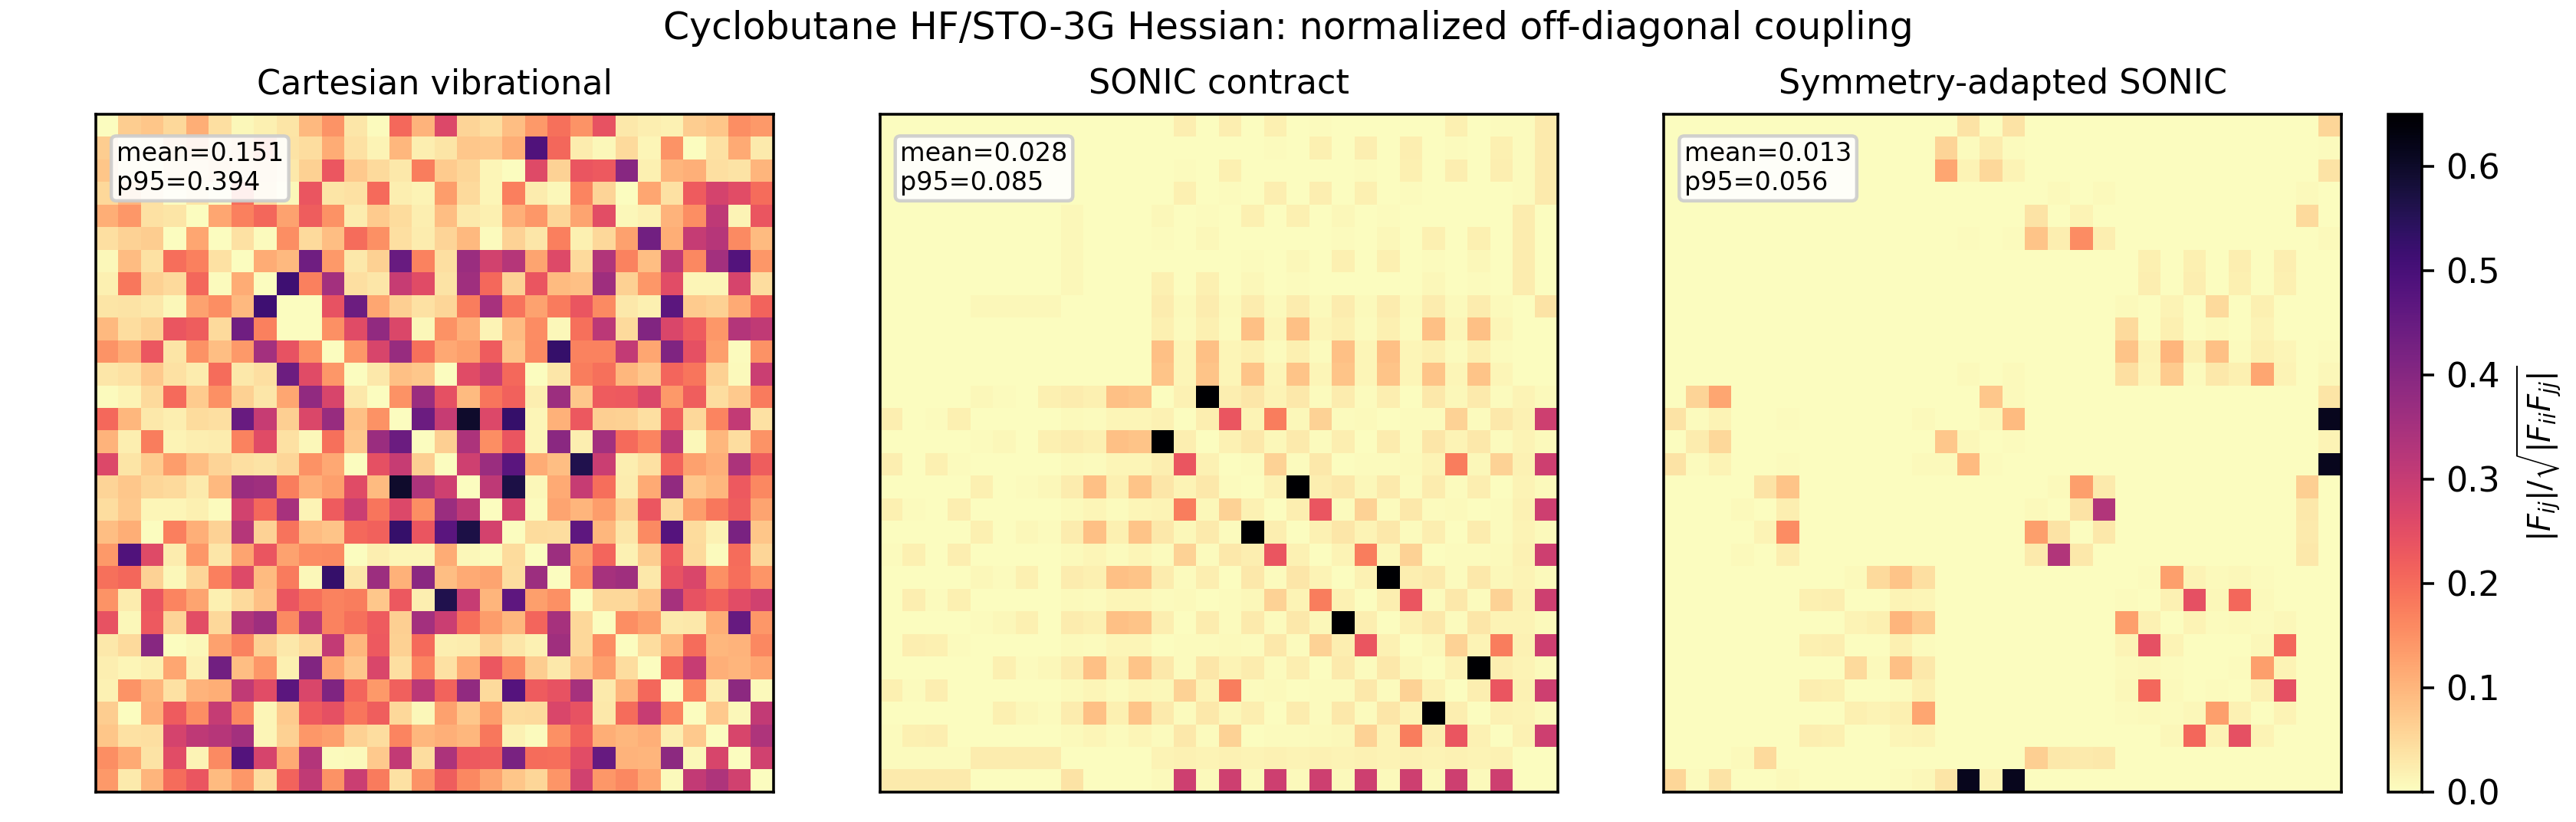
\includegraphics[width=\linewidth]{figures/neo_hessian_heatmap.png}
\caption{Normalized off-diagonal Hessian coupling for cyclobutane
(Gaussian DV HF/STO-3G).  The same Cartesian Hessian is represented in an
orthonormal Cartesian vibrational basis, in the frozen \NEO\ contract and in the
symmetry-adapted \NEO\ contract.  The diagonal is suppressed so that residual
coordinate coupling is visible.}
\label{fig:hessian-heatmap}
\end{figure}

\subsection{GF/PED Family Scaling Probe}

A Wilson GF/PED calculation is the most direct spectroscopic test of whether the
coordinate families produced by \NEO\ remain chemically readable after
projection.  In scaled-quantum-mechanical force-field work, force constants are
often adjusted by coordinate class rather than by individual normal
modes.\cite{RauhutPulay1995,BakerJarzeckiPulay1998,BaroneBiczyskoBloino2014}
That operation is only transparent when the coordinate blocks keep stretches,
bends, torsions and ring-puckering coordinates separated.

The add-on test uses cyclohexanol at GDV B3LYP/6-31G(d), with standard
\texttt{Opt Freq NoSymm} and no out-of-plane GIC terms.  \NEO\ supplies the
frozen coordinate contract and sparse \(\Bmat\) rows; the GF layer then applies
family-level Pulay-style scale factors to the internal force field and reports
PED percentages by source family.  The contract has rank \(51/51\).  The
unscaled GF frequencies reproduce the Gaussian/FCHK harmonic frequencies with
an RMS difference of \(2.6\times10^{-6}\)~cm\(^{-1}\), and the aligned
optimized geometry agrees to \(4.7\times10^{-7}\)~\AA.  The hydroxyl stretch is
deliberately assigned a force-constant factor larger than one, corresponding to
an approximately \(+100\)~cm\(^{-1}\) shift, because localized OH stretches are
a known sensitive region for modest harmonic DFT levels and are usually treated
by class-specific calibration rather than by a single global frequency scale
factor.

\begin{table}[htbp]
\centering
\caption{Representative GDV B3LYP/6-31G(d) GF/PED scaling probe for
cyclohexanol.  Frequencies are in cm\(^{-1}\).  PED entries are summed over
\NEO\ coordinate families and rounded to one decimal percent.}
\label{tab:gf-ped-scaling}
\begin{tabular}{@{}p{0.24\linewidth}ccp{0.42\linewidth}@{}}
\toprule
Representative mode & Unscaled & Scaled & Dominant PED families \\
\midrule
Low-frequency ring deformation & 269.158 & 266.496 & Heavy stretch 49.8; ring puckering 25.0; bend/rock 21.9. \\
Ring bend/deformation & 475.915 & 472.567 & Heavy stretch 58.1; ring bend 27.3; bend/rock 13.7. \\
Heavy-atom stretch/bend & 1106.899 & 1104.650 & Heavy stretch 89.2; bend/rock 10.5. \\
CH stretch & 3088.189 & 3033.689 & CH stretch 100.0. \\
OH stretch & 3748.716 & 3850.456 & OH stretch 99.9. \\
\bottomrule
\end{tabular}
\end{table}

The large-amplitude block analysis is consistent with the same family
separation: the torsion block gives 270.542~cm\(^{-1}\), while the three
ring-puckering rows give 224.217, 417.617 and 473.078~cm\(^{-1}\).  The active
DVR candidate is the \(RPck0003\) row at 225.084~cm\(^{-1}\).  This is the
spectroscopic counterpart of the construction principle: scaling classes are
assigned to \NEO\ family labels such as \texttt{Stre0012}, \texttt{RPck0002}
or \texttt{RDef0026}, not to handwritten normal-mode descriptions.

\subsection{Ring Puckering Branch}

This probe uses the same cyclobutane contract to define a one-dimensional
ring-puckering branch.  The coordinate is the alternating carbon-ring puckering
amplitude associated with the \(D_{2d}\) ring source block.  Single-point
Gaussian DV HF/STO-3G energies were evaluated along a fixed substituent-frame
branch.  This is intentionally not a relaxed conformational profile; it is a
test that a named puckering coordinate can be used as a reproducible sampling
axis while the contract retains the same ring-source identity.

Figure~\ref{fig:puckering-scan} illustrates the result.  The minimum on this
fixed branch is near \(q=0.04\)~\AA, matching the optimized reference
geometry.  Larger puckering displacements raise the energy smoothly.  In a DVR
or PES-fitting application, the same base coordinate could be replaced by a
Cremer--Pople amplitude or phase function \(y=f(\q)\), while the analytic
chain-rule row would still descend from the frozen \NEO\ \(\Bmat\).

\begin{figure}[htbp]
\centering
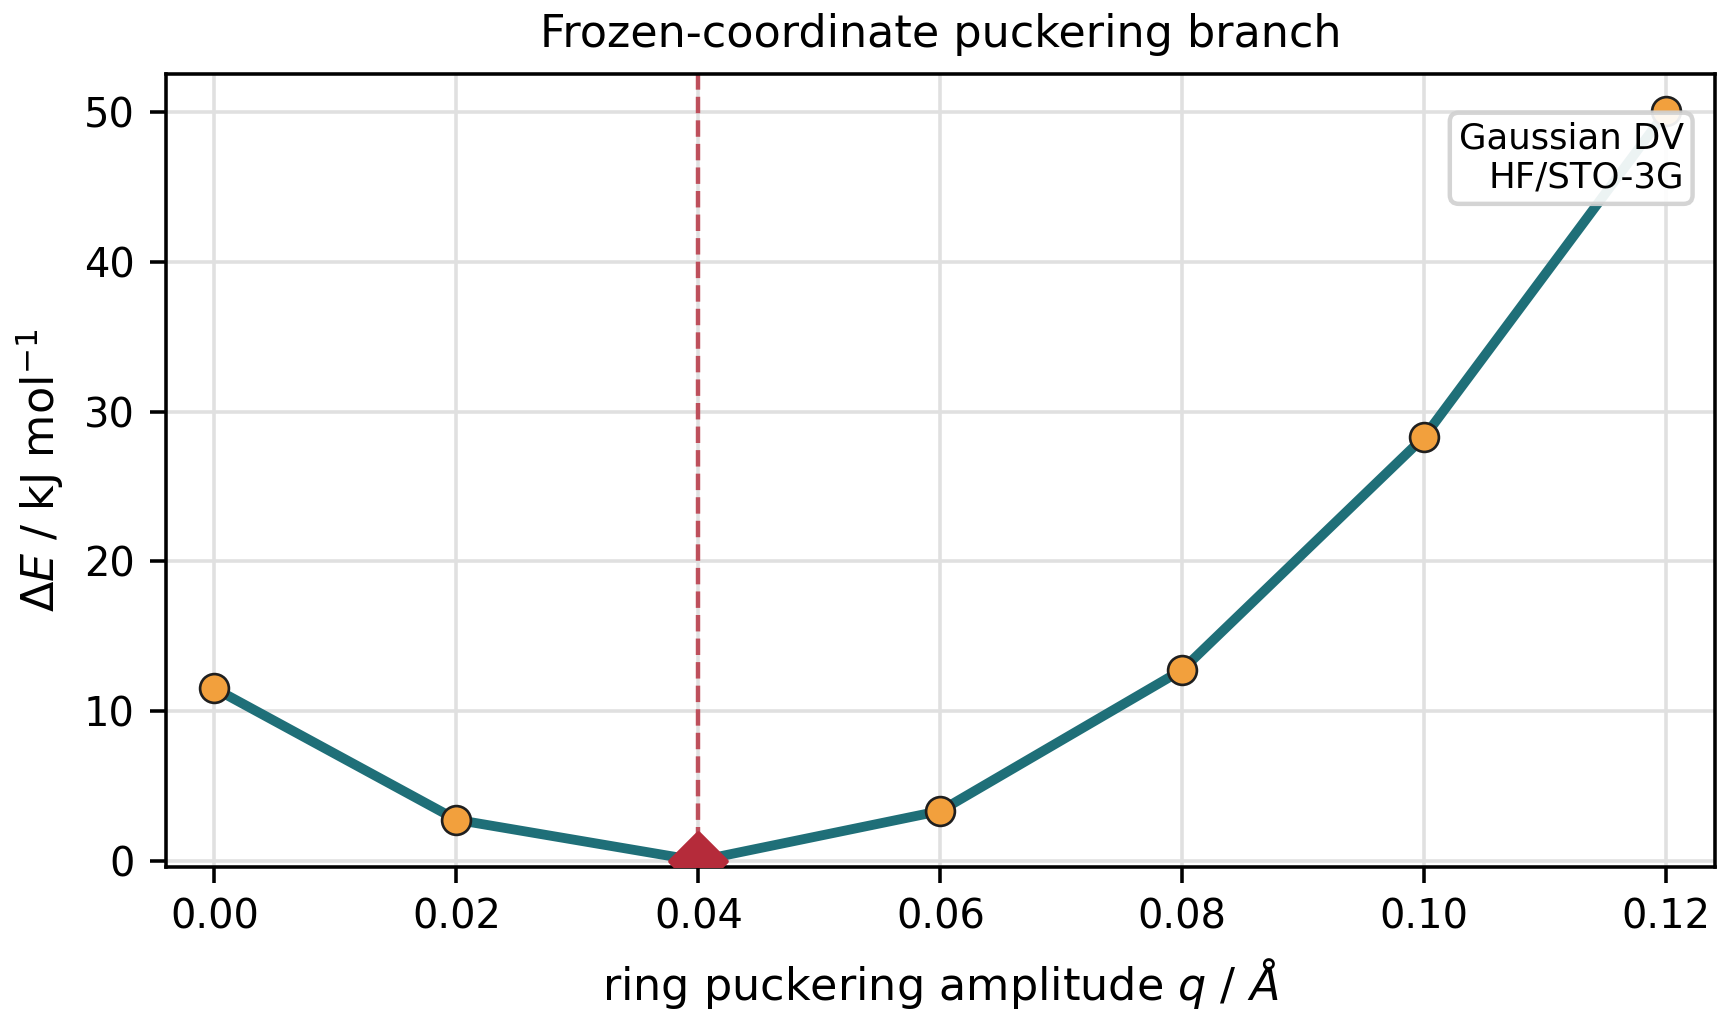
\includegraphics[width=0.68\linewidth]{figures/neo_puckering_scan.png}
\caption{Fixed-frame cyclobutane puckering branch generated from the frozen
\NEO\ ring coordinate and evaluated with Gaussian DV HF/STO-3G single-point
energies.  The branch is a coordinate diagnostic, not a relaxed conformational
energy profile.}
\label{fig:puckering-scan}
\end{figure}

\subsection{Portable Chair-to-Boat Puckering Export}

The final probe tests a stricter export question, using the same cyclohexane
ring-flip motif discussed in the Gaussian GIC paper and its Supporting
Information.  There, the puckering coordinate is encoded by an explicit
molecule-specific input block containing variables such as \texttt{Gcyc},
\texttt{Ccyc} and \texttt{Scn0}.  Here no such block is provided.  \NEO\ starts
from the molecular graph and geometry, generates the ring-puckering contract,
and then constructs a fixed-frame cyclohexane puckering path from the chair
\(q_3\) component to the boat \(q_2\) component.  For each point it generated
two independent external representations of the same geometry: a portable
Cartesian input, usable by any electronic-structure program, and a Gaussian
\texttt{ReadAllGIC} input containing the automatically generated coordinate
contract.  Gaussian DV B3LYP/6-31+G* single-point energies were then evaluated
from both inputs.

All five contracts have rank \(48/48\) and contain no out-of-plane GIC terms, so
the comparison uses only syntax supported by standard Gaussian
\texttt{ReadAllGIC}.  Figure~\ref{fig:cyclohexane-puckering-equivalence} shows
that the two energy traces are numerically identical: the largest
Cartesian--\texttt{ReadAllGIC} difference is \(3.0\times10^{-3}\,\mu E_h\),
about \(8\times10^{-6}\)~kJ~mol\(^{-1}\).  The large rise along the path is not
a chair--boat barrier; it is the expected cost of an unrelaxed fixed-frame
puckering deformation.  The result instead shows that the same \NEO{}-generated
large-amplitude coordinate path can be exported either as ordinary Cartesians or
as an automatically generated Gaussian GIC model without changing the electronic
energy surface being sampled.

Because the Cartesian branch is ordinary molecular geometry, it is not tied to
Gaussian.  The same three representative points were also evaluated on the
Oracle machine with ORCA and Molpro at PBE0/def2-SVP, a different level from
the B3LYP/6-31+G* Gaussian check.  The absolute energies differ slightly
between codes, as expected from independent DFT implementations and defaults,
but the relative fixed-frame puckering profile is the same at the level needed
for this export test (Table~\ref{tab:external-codes}).  This verifies the
intended division of labor: \NEO\ constructs the model and coordinates, while
external electronic-structure programs consume the resulting Cartesian
geometries or GIC serializations.  It confirms that the coordinate contract is
independent of the electronic-structure implementation.

\begin{table}[htbp]
\centering
\caption{Portable cyclohexane puckering coordinates evaluated by non-Gaussian
codes on Oracle.  Energies are PBE0/def2-SVP single points on the same
\NEO{}-generated Cartesian geometries; relative energies are in kJ mol\(^{-1}\)
with respect to \(p00\).}
\label{tab:external-codes}
\begin{tabular}{lrrrr}
\toprule
Point & ORCA \(E_h\) & ORCA \(\Delta E\) & Molpro \(E_h\) & Molpro \(\Delta E\) \\
\midrule
\(p00\) & -235.422463982 & 0.000 & -235.422142275 & 0.000 \\
\(p02\) & -235.321345943 & 265.485 & -235.321038853 & 265.447 \\
\(p04\) & -235.103704314 & 836.903 & -235.103335256 & 837.028 \\
\bottomrule
\end{tabular}
\end{table}

\begin{figure}[htbp]
\centering
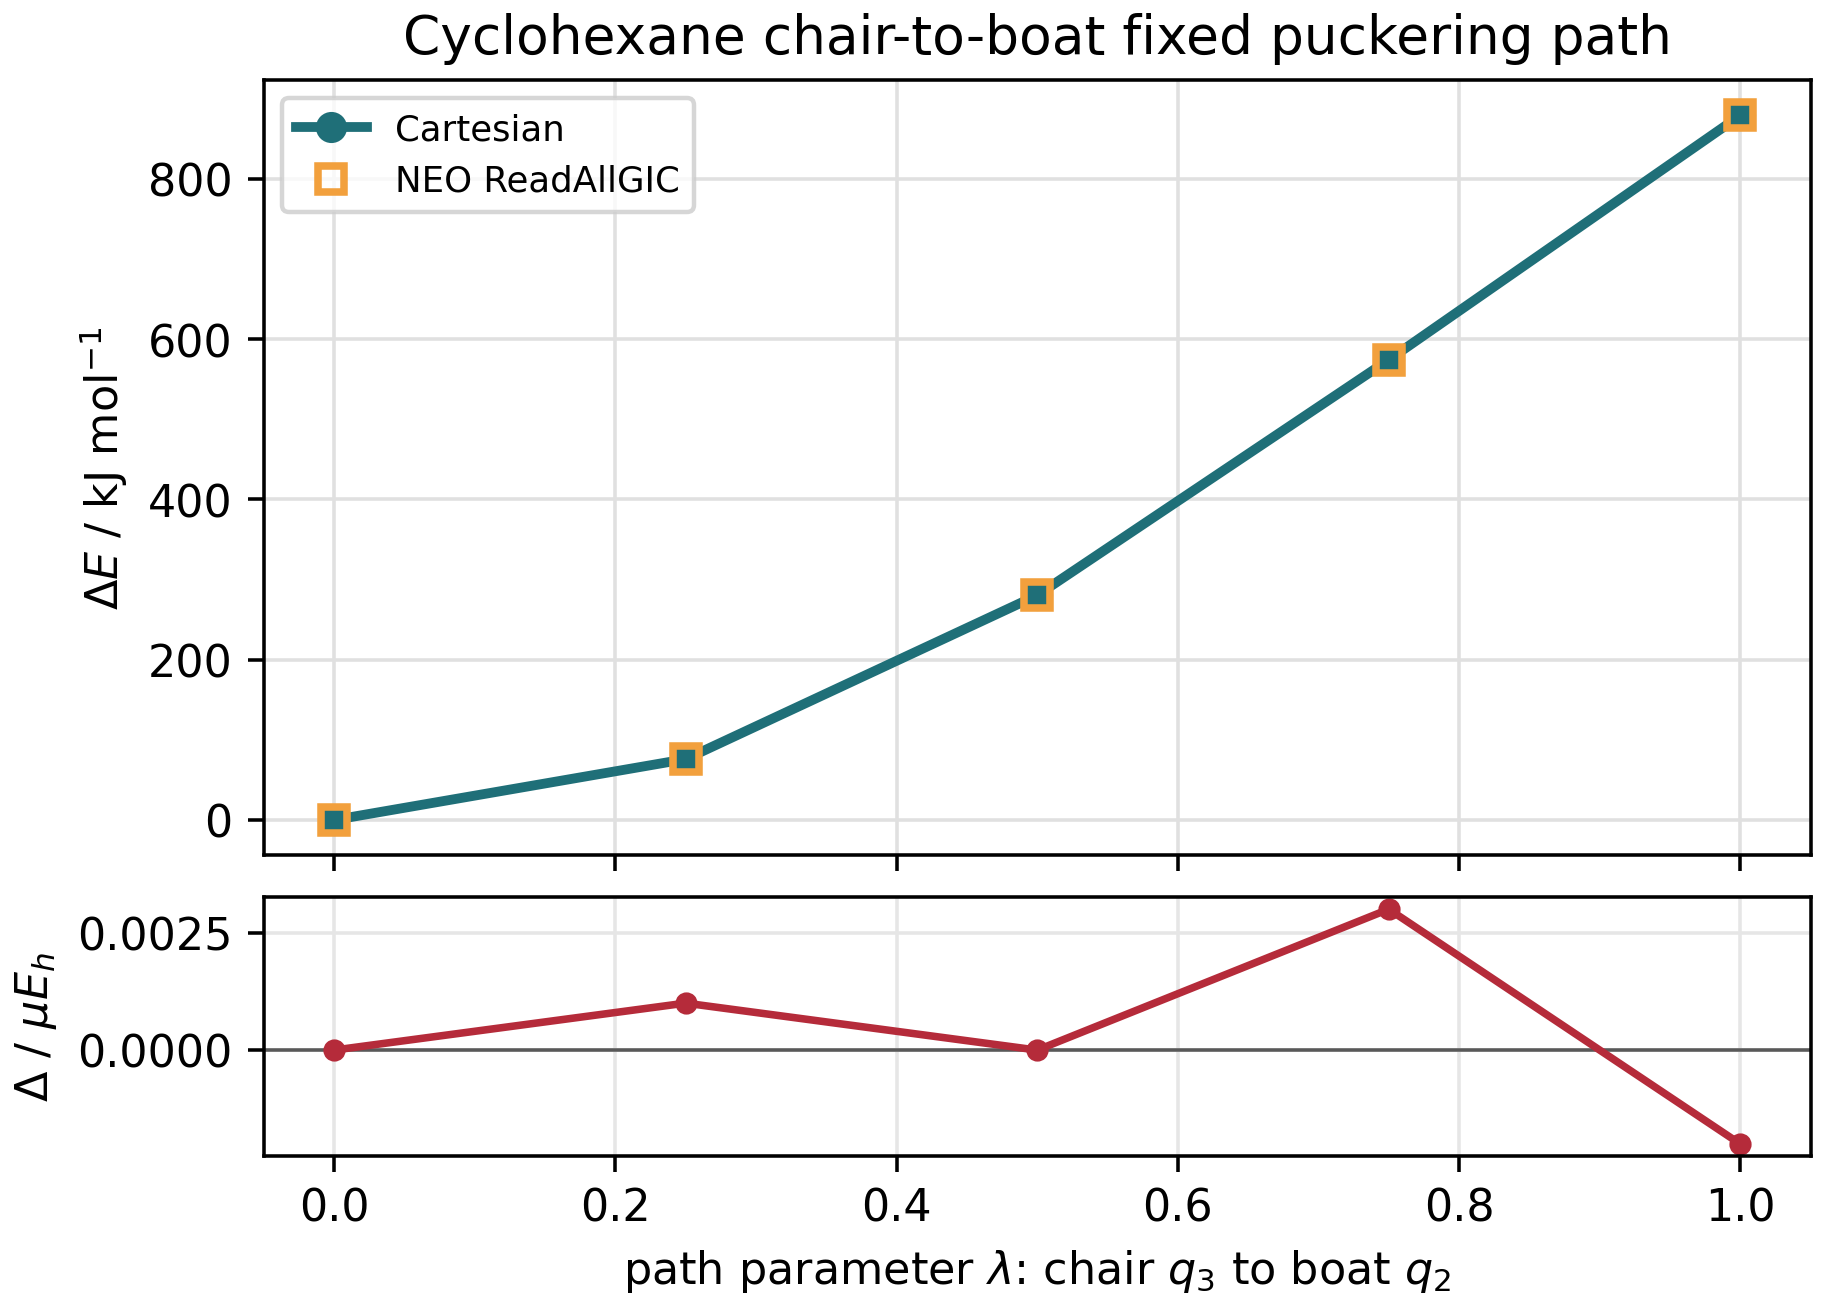
\includegraphics[width=0.78\linewidth]{figures/cyclohexane_puckering_equivalence.png}
\caption{Cyclohexane fixed-frame chair-to-boat puckering export test
(Gaussian DV B3LYP/6-31+G*).  The upper panel compares the same five geometries
evaluated from portable Cartesian inputs and from \NEO{}-generated
\texttt{ReadAllGIC} inputs.  The lower panel gives the energy difference in
microhartree.}
\label{fig:cyclohexane-puckering-equivalence}
\end{figure}

\section{Discussion}

\NEO\ can be viewed as a constructive generalization of natural internal
coordinates.  Its novelty is not the use of Wilson rows, SVD, Gram--Schmidt or
SALC projectors individually.  Its novelty is the deterministic protocol that
builds a non-redundant basis while respecting locality, symmetry, semantic
priority, protected special coordinates, ring source spaces and fragment
coordinates in one frozen contract.  The same generator handles ordinary
valence coordinates, ring puckering components, butterfly torsions,
high-coordination angular blocks, fragment translations, fragment orientations
and center-based distances.  The method is deliberately not a single global
orthogonalization.  It is a sequence of local and block-local decisions followed
by a rank audit in the physical Wilson \(\Bmat\)-row space.
The compact structural observations above are intentionally modest: \NEO\ is
natural with respect to symmetry-preserving relabellings, the contract is
deterministic on a frozen state, protected semantic coordinates are retained
whenever rank compatibility allows them, block-local reduction is insensitive
to homogeneous scaling, and the discrete contract is locally stable inside a
fixed molecular-state stratum.  Each point follows directly from the fixed
candidate order, normalized Gram--Schmidt rank tests and homogeneous
point-group projectors described in Sec.~6--7.

The method should therefore be read as a documented coordinate-selection
protocol, not as a proof that only one internal-coordinate basis is possible.
Normalized Wilson-row testing removes the most direct dependence on raw physical
units in the final rank decision, but the protected-first family order remains a
chemical modelling choice.  The point is that this choice is explicit,
reproducible and reported, rather than hidden in primitive weights chosen before
a global diagonalization.

This is also the practical answer to the possible ``black box'' criticism.
The output of \NEO\ is not an undocumented list of optimizer variables.  It is a
frozen coordinate contract with primitive definitions, coefficients, family
labels, irreducible representations, rank diagnostics and analytic derivative
rows.  Moreover, downstream calculations can compare the \GIC\ active space
with a symmetry-adapted Cartesian nullspace that is not built from GIC
primitives.  Agreement between the two active spaces shows that the chemical
conclusion does not depend on a hidden choice inside the coordinate generator,
but on the shared topology, symmetry and rank of the molecular problem.

The internal validation in Table~\ref{tab:validation} establishes rank closure,
symmetry-projector normalization and Python--Fortran row-space equivalence for
representative cases.  This is an implementation-level cross-check inside the
\ORACLE\ development lineage, not a comparison with an external published
natural-coordinate program.  Table~\ref{tab:frisch-si} addresses the more
external-facing question raised by the Gaussian GIC Supporting Information: can
the same kinds of chemically specialized variables be generated without
hand-writing molecule-specific GIC expressions?  Gaussian supplies a powerful
expression and derivative language; \NEO\ supplies automatic construction,
semantic interning of generated coordinates, sparse derivative propagation and
frozen provenance.  In this sense, GIC syntax is a serialization and solver
interface for \NEO, not a competing coordinate-generation theory.  The
cyclohexane check makes this distinction concrete: the Gaussian-style puckering
model is available to the external solver, but its coordinate definitions are
not typed by hand.

\subsection{Computational Cost and Remaining Validation}

The computational separation is the same as the conceptual separation.  The
coordinate contract is constructed once for a frozen molecular state; only the
analytic \(\Bmat\) rows and derived coordinate functions need to be evaluated
again at later optimization, scan, GF/PED or refinement geometries.  If \(m\) is the
number of primitive candidates, \(r\) the target rank and \(z\) the number of
nonzero sparse derivative entries, the current dense rank audit scales as
\(O(mr\,3N)\) for modified Gram--Schmidt after the local block reductions have
been formed.  For ordinary molecular graphs \(m\) and \(r\) are both linear in
\(N\), so this one-time audit has cubic worst-case dense scaling but remains a
build-time cost.  The per-geometry derivative service is sparse and scales with
\(z\), plus the sparse chain-rule cost for any derived functions.  Large fused
ring systems, high-coordination templates and fragment special coordinates add
block-local SVD or projector work, but these operations are confined to their
homogeneous source blocks rather than to a global primitive matrix.  A timed
scaling benchmark is not yet included and should be added before treating
performance as a validated claim.

Several validation items also remain intentionally open.  The local-stability statement gives an existence threshold
\(\delta\) in terms of decision margins \(\mu_a\) and Lipschitz constants
\(L_a\), but the present draft does not report a numerical \(\delta\), \(\mu_a\)
or \(L_a\) for a real molecule.  A future validation table should instantiate
these quantities for representative systems, at least at the level of finite
difference lower bounds on decision margins and empirical Lipschitz estimates
inside a fixed topology/symmetry stratum.  The same caveat applies to
point-group perception near borderline geometries: determinism is guaranteed
for the frozen \ORACLE\ state, but an unconstrained optimization that moves
back and forth across a symmetry tolerance can legitimately produce different
frozen strata.  The implementation records point-operation residuals and the
minimum residual margin against the stored symmetry tolerance, and flags
near-threshold operations in the frozen coordinate contract; quantitative
tolerance-sensitivity
tables are part of the roadmap rather than a claim made by the present
validation.  Likewise, the manuscript does not yet compare \NEO\ against an
external published natural-coordinate generator; the Gaussian tests are export
and solver-consumption tests, not an external coordinate-generator benchmark.
The protected-prefix rejection rule is covered in the semantic coordinate layer
unit probes in Table~\ref{tab:validation}; a chemically realistic
overconstrained example remains a useful future diagnostic.

The main limitation is no longer the absence of pseudo-bonds in the code path,
but the current validated scope of the pseudo-cycle tests.  Protected fragment
and special-center coordinates are already suitable for weak complexes and
coordination motifs, while the pseudo-bond baseline covers typed hydrogen-bond
closures and bifurcated contacts.  What remains to be expanded is the corpus of
symmetry-rich intermolecular cycles and the numerical stress testing of those
pseudo-cycle rows under geometry changes.

\subsection{Scope and Limitations}
\label{sec:scope-limitations}

\NEO\ is intended for high-accuracy quantum-chemical, spectroscopic and
refinement workflows in which the coordinate model carries chemical information
and must be reused across modules.  It is not designed as a large-scale
thousand-atom molecular-dynamics coordinate generator, a generic classical
force-field engine or a machine-learning featurizer.  Users who need a frozen,
auditable, symmetry-aware coordinate contract for molecules, rings, fragments
or coordination motifs are the target audience; users who only need a
black-box optimizer coordinate for very large systems should normally use a
lighter optimizer-specific representation.

The construction is conditional on a fixed molecular-state stratum.  Bond
breaking or forming, proton transfer that changes the covalent graph, and
coordination rearrangements require separate contracts or a future
state-interpolation model.  An EVB-like or subspace-interpolation layer may be
possible, but it is not part of the present theory.

The Wilson rows used here are first-order derivatives at the frozen geometry.
Large distortions along scans, optimizations or refinement trajectories may
require recomputing the \(\Bmat\) rows or decomposing a large transformation
into smaller steps.  A future adaptive update could preserve the semantic
contract while refreshing local derivative information, but the present draft
does not validate such an update scheme.

The protected-first rule is a chemically motivated modelling principle, not a
mathematical uniqueness theorem over all possible coordinate bases.  Alternative
priority orders would define different, still reproducible contracts.  The
claim made here is that the priority order is explicit, versioned and
diagnosed, and that protected coordinates are not silently displaced by
ordinary coordinates when they are compatible with the target rank.

Finally, determinism is conditional on the frozen \ORACLE\ state:
geometry, topology, symmetry operations, continuous atom perception, synthon
descriptors, tolerances, semantic grammar version and contract schema version.
A different perception model or tolerance policy may produce a different
contract; the scientific requirement is that such a change is visible in the
provenance rather than hidden in an implementation choice.

\section{Conclusions}

\NEO\ provides a general, frozen and symmetry-aware construction of
generalized internal coordinates for \ORACLE.  Its main contribution is a
deterministic coordinate contract that integrates ingredients usually treated
separately: natural-coordinate locality, analytic Wilson-\(\Bmat\) rank control,
homogeneous point-group symmetrization and protected special coordinates for
rings, fragments and interaction centers.  This is the coordinate object
intended for reuse across Gaussian input generation, GF/PED vibrational scaling
and force-field analysis, large-amplitude DVR grids, PES fitting,
semi-experimental refinement and workflow diagnostics.
Nonlinear coordinate functions such as inverse or exponential distances,
trigonometric angular terms and Cremer--Pople descriptors can be built on top of
this base by analytic chain-rule differentiation.

The present construction supports the intramolecular machinery needed for
acyclic, cyclic, fused, bridged, spiro and high-symmetry molecules, together
with special-coordinate and pseudo-bond models for weak complexes within the
validated baseline described above.  The next methodological step is to enlarge
the pseudo-cycle validation corpus for intermolecular systems, using the same
rank, symmetry and analytic-\(\Bmat\) invariants used by the rest of \NEO.
The Gaussian \texttt{ReadAllGIC} optimization probes show that the present
contract is already usable as an external solver coordinate set.  The Hessian,
puckering, GF/PED scaling and portable chair-to-boat export probes illustrate
why the same contract is relevant to force-field and large-amplitude work
within the scope defined above.  Full DVR and refinement application benchmarks
remain the next validation layer.  The cyclohexane export check further shows
that a \NEO{}-generated puckering path can be represented either as ordinary
Cartesians or as Gaussian \texttt{ReadAllGIC} input with numerically identical
energies.

\section*{Reproducibility}

The calculations reported in the validation and application sections were
generated with the \NEO\ development tree and Python 3.13.11.  Gaussian
jobs used the local Gaussian DV executable documented in the accompanying
scripts; the method and basis set are stated with each probe.  The reported
construction tests are deterministic and do not use stochastic seeds.  The
Python implementation is checked against a separate Fortran control
implementation for the corpus rows where that comparison is applicable.

\section*{Data and Code Availability}

The manuscript repository contains the scripts, JSON data files and figures
used to generate the tables and application plots.  The \NEO\ source
code is under active development and will be released with the \ORACLE\
distribution; until public release, the code and frozen input/output data are
available from the author upon reasonable request.

\section*{Author Contributions}

Vincenzo Barone conceived the method, designed the \NEO\ coordinate
contract, implemented the active code paths used here, performed the
calculations and wrote the manuscript.  External refinement and PES-fitting
consumers are discussed only as downstream uses of the coordinate contract.

\section*{Acknowledgments}

The author acknowledges the broader \ORACLE\ development environment used to
test the coordinate contracts, the Gaussian GIC work that motivated the
distinction between coordinate-description languages and automatic generation,
and the ring-reconstruction work of Lema-Saavedra and Fern{\'a}ndez-Ramos that
clarified how puckering coordinates connect to closed molecular geometries.

\bibliographystyle{unsrtnat}
\bibliography{references}

\end{document}
